% \documentclass[%
%  reprint,
%  amsmath,amssymb,
%  aps,
% ]{revtex4-2}
\documentclass[%
 reprint,
 amsmath,amssymb
 aps,
]{revtex4-2}

\usepackage{float}

\usepackage{graphicx}% Include figure files
\usepackage{dcolumn}% Align table columns on decimal point
\usepackage{bm}% bold math
\usepackage{physics}
\setlength{\parskip}{\baselineskip}%
\usepackage{siunitx}
\usepackage[inline]{asymptote}
\usepackage{multirow}
\usepackage{tikz}
\usepackage{pgfplots, pgfplotstable}
% \def\bibsection{\section*{\refname}} 
\usepackage{hyperref}
\usepackage{natbib}
\bibliographystyle{unsrtnat}

\pgfplotsset{compat=1.3}
\begin{document}

% \preprint{APS}

\title{Determining the Q Factor of a Homemade Pendulum}% Force line breaks with \\

\author{QiLin Xue}

\date{\today}% It is always \today, today,
             %  but any date may be explicitly specified

\begin{abstract}
This paper will present the results of how air resistance, amplitude, length, and mass affects the motion of a homemade pendulum. The results are compared against a simplified model of dampened harmonic motion often taught in physics classes, and deviations are analyzed by examining more realistic effects such as laminar versus turbulent flow, large amplitudes, and effects that arise from the irregular shape of the water bottle used as a pendulum. These were performed in various experiments, each changing only one of the above factors. The results show that generally, the model taught in schools give reasonable predictions but there are elements that can be improved.
\end{abstract}

%\keywords{Suggested keywords}%Use showkeys class option if keyword
                              %display desired
\maketitle

% \tableofcontents
\section{Introduction}

Pendulums have been used since the 17th century to keep track of time.\cite{pendulum} Their design is extremely simple: they generally consist of a small but heavy mass connected at the end of a long freely rotating rod. One useful characteristic is that for small angles, the period of motion is not ``greatly'' affected by external factors such as air resistance and the initial angle. In this report, we will attempt to quantify effects such as air resistance, angle, mass, and length to see how much variation in these parameters affect the motion of a pendulum.
\subsection{Air Resistance}
As a result, it is extremely important to analyze how the amplitude decreases due to air resistance, the major contributing effect. Assuming a linear drag of $F_d=-bv$ and approximating the pendulum as a point mass, the net torque gives the differential equation:
\begin{equation}
    \frac{d^2\theta}{dt^2} + \frac{b}{m}\frac{d\theta}{dt} + \frac{g}{\ell}\theta  = 0
\end{equation}
where the small angle approximation $\sin\theta\approx\theta$ has been used. There are a variety of factors affecting the behaviour of this system, and to solve it for the most general case we can nondimensionalize this equation with the substitution $t=T\left(2\pi \sqrt{\frac{\ell}{g}}\right)$ where $T$ is a dimensionless number that represents the number of periods. Substituting this in, we get:
\begin{equation}
    \frac{g}{4\pi^2\ell}\frac{d^2\theta}{dT^2}+\frac{b}{2\pi m}\sqrt{\frac{g}{\ell}}\frac{d\theta}{dT}+\frac{g}{\ell}\theta = 0
    \label{eq:}
\end{equation}
which can be written in the form of
\begin{equation}
    \frac{d^2\theta}{dT^2}+2\pi Q\frac{d\theta}{dT}+4\pi^2\theta = 0
    \label{eq:}
\end{equation}
where we have defined a new dimensionless number known as the quality factor and given by $Q\equiv \frac{b}{m}\sqrt{\frac{\ell}{g}}$. The solution to this equation is well known (see Appendix A) and is given by:
\begin{equation}
    \theta = \theta_0e^{-\pi QT}\cos\left(2\pi T + \phi\right)
    \label{eq:}
\end{equation}
where $\theta_0$ is the initial angle, $\phi$ is the phase shift, and all quantities are dimensionless numbers. The first factor $\theta_0e^{-\pi QT}$ is known as the envelope function and qualitatively it describes how the amplitude changes with time. If the amplitude is to change by a factor of $e^{-\pi/N}$, then we have:
\begin{equation}
    \theta_0e^{-\pi/N}=\theta_0e^{-\pi QT} \implies T = \frac{Q}{N}
    \label{eq:}
\end{equation}
If $N=2$, then by counting how many periods it takes for the amplitude to change by a factor of $e^{-\pi/2}\approx 21\%$ gives the quantity $Q/2$. Alternatively, by numerically fitting experimental data with the the model also allows $Q$ to be extracted.

\subsection{Angle Dependance}
For large $Q$ values, the amplitude would decay very slowly. However, the physical interpretation of the $Q$ value only applies for small angles so we also wish to examine what happens at larger angles. In reality, the period is dependant on the amplitude $\theta_0$ via the relationship:\cite{doi:10.1119/1.1457310} %CITE
\begin{equation}
    T = 2\pi\sqrt{\frac{\ell}{g}}\left(1+\frac{1}{16}\theta_0^2+\frac{11}{3072}\theta_0^4+\cdots\right)
    \label{eq:correct-model}
\end{equation}
where $\ell$ is the distance from the center of mass of the pendulum to the pivot.

\subsection{Length and Mass Dependance}
We shall also consider the fact that no pendulum can be a point mass\footnote{It's not ``just'' a \href{https://youtu.be/kmgwYrwJ3M8?t=129}{swinging delta function}}. Therefore, while the previous approximations states that the period of a pendulum is directly proportional to the square root of the length of string, this is not an entirely true model.

For a compound pendulum, the period is given by:
\begin{equation}
    T = 2\pi\sqrt{\frac{I}{mg\ell_\text{cm}}}
    \label{eq:}
\end{equation}
If the moment of inertia of the water bottle around the center of mass is $I_\text{cm}=\beta m d^2$ where $d$ is the length of the water bottle, then by the parallel axis theorem, the period can be written as:
\begin{equation}
    T = 2\pi\sqrt{\frac{\beta d^2 + \ell_\text{cm}^2}{g\ell_\text{cm}}}
    \label{eq:proper}
\end{equation}
A nicer form to work with would be the lowest order approximation
\begin{equation}
    T = 2\pi\sqrt{\frac{\ell_\text{cm}}{g}}\left(1+\frac{\beta d^2}{2\ell_\text{cm}^2}\right)
    \label{eq:low order}
\end{equation}
Since mass does not appear in this equation, I would not expect the period to be affected by increasing the mass if all other quantities are the same.

\section{Method}
With the exception of measuring the length dependance, all experiments were performed with similar setups. Specific details and changes are explained in their respective subsections. Two light strings with a mass smaller than $ <0.5\si{\gram}$ were used to hang a small plastic water bottle from a nail drilled into a wall using two strings, one on each side of the bottle. Figure \ref{fig:bottle} shows the shape and dimensions of the water bottle, measured with a metre stick.
\begin{figure}[!h]
    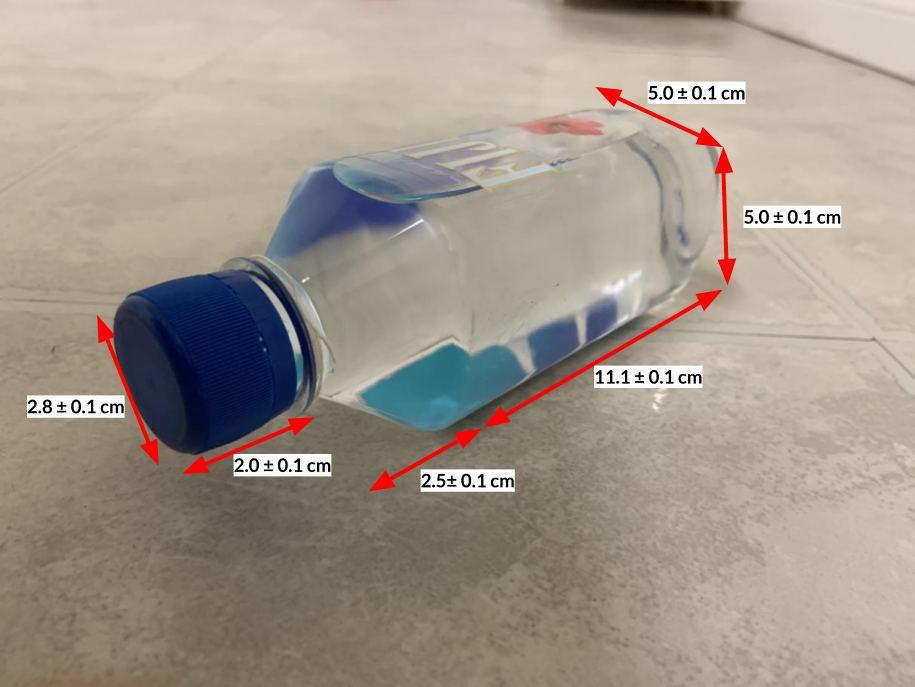
\includegraphics[width=\linewidth]{figures/bottle.png}
    \caption{Dimensions of the water bottle used. It can be approximated as a rectangular prism attached to a trapezoidal pyramid and a cylinder. Note that due to the camera angle, the lengths drawn in the picture are not to scale.}
    \label{fig:bottle}
\end{figure}
A High Definition 720p 120fps GoPro Hero 4 Silver camera was used, set to ``linear mode.'', and placed a large distance away from the equilibrium position of the pendulum. Another string was hung and offset to the side to act as a reference marker to ensure the pendulum was swinging in the plane parallel to the wall. I slowly provided the pendulum a small angular displacement using this string as a reference, released it from rest, and let it run until either the swinging was barely noticeable or until enough data has been obtained. The setup is shown in figure \ref{fig:setup}.
\begin{figure}[!h]
    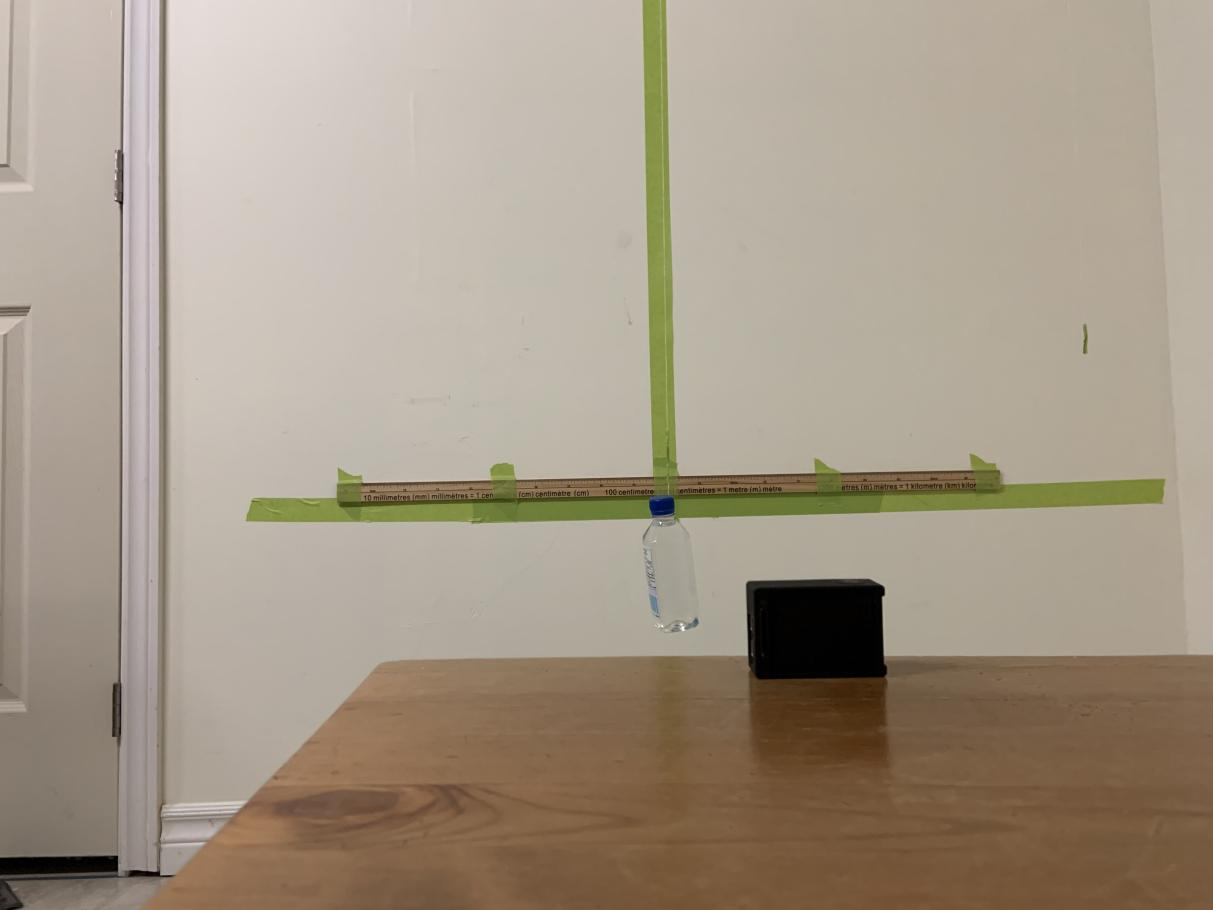
\includegraphics[width=\linewidth]{setup.jpg}
    \caption{A water bottle is tied to a light string hung above (out of frame). A ruler is taped to the wall, and green tape runs directly behind the string to make it easier for the GoPro to be lined up. A second string with tape on its end hangs towards the side. In the setup used for the experiment, an extra string was added to ensure the orientation stays constant.}
    \label{fig:setup}
\end{figure}
The position of the pendulum in each frame was obtained using the \textit{AutoTracker} feature of the \textit{Tracker} software\cite{tracker}, a free online tool that can estimate the location of a marker via kinematic data and pixel comparison. A meter stick was taped in the background to calibrate the distances in the software. The collected raw data was then processed through my own customized Python script (see Appendix B) to extract the useful information.
\subsection{Q Factor and Angle Dependance}
The length of the string for this first experiment was $107.5 \pm 0.1\si{\centi\meter}$, with an estimated center of mass a distance $7 \pm 1\si{\centi\meter}$ away from the string, which is derived in the Discussion section.

The $Q$ factor and the angle dependance was measured using the same experiment. The initial angle was set to near $90^\circ$, and was left to swing until it was nearly stopped. The camera was set very far away in order to capture the entire motion of the pendulum. Because of this, no optical corrections were found to be necessary.

As the amplitude decreases, it is predicted that the period would decrease as well. To reduce time uncertainties and statistical fluctuations, half-period measurements were made by measuring the time over a small intervals of amplitudes each with a range of $\Delta \theta = 0.2$. By finding the average of these half-amplitude measurements, I can get an estimate for the period at the midpoint (e.g. the average amplitude in each interval).

Even though this increases the uncertainty in the amplitude, the motivation is that for any small variation in the amplitude, the period can be approximated as linear with respect to amplitude such that a higher period from a higher amplitude would balance out the lower period from a lower amplitude, to arrive at a fairly accurate and precise average. In other words, if we sum up all period measurements that fall inside the interval $[\theta,\theta+0.2]$, the average period gives the period at the midpoint. All calculations along with error propagation was done in a Python notebook.

Once the relationship has been experimentally verified, a range of angles in which the effects of the amplitude are no longer important was determined. Using this information, the $Q$ factor was measured by looking at the motion of the pendulum in this range to verify that the effects of air resistance is relatively small.
\subsection{Length and Mass Dependance}
In order to make it easier to change length, the pendulum was attached to a pulley system as shown in figure \ref{fig:cool}. As the bottle swings, the other end of the pulley was pulled down such that the length changes roughly adiabatically (slowly, no external torques are applied). A GoPro camera was used to record at 120 fps, such that the time uncertainty for a single oscillation is $\delta t = 0.004 \si{\second}$, which is equal to the uncertainty if I had manually timed it for ten oscillations. As a result, by slowly and continuously changing the length, I was able to get period measurements for $200$ different lengths to a good precision. These measurements were then grouped together into $40$ data points by taking the average of consecutive five trials.
\begin{figure}[!h]
    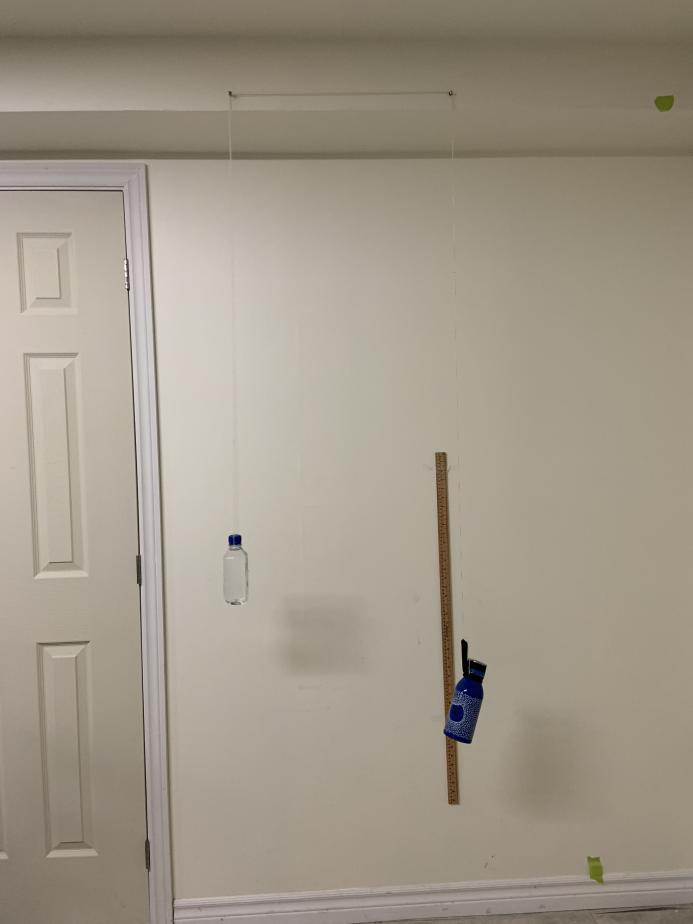
\includegraphics[width=\linewidth]{figures/cool_beans.jpg}

    \caption{The modified pendulum setup. Another mass is tied to the right end, which allowed it to easily change the length of the swinging pendulum (left). A ruler is taped in the background for calibration purposes.}
    \label{fig:cool}
\end{figure}
Unfortunately, there was no easy way to change the mass so the oscillations were recorded manually. The mass of the pendulum was changed by dumping out small portions of the water after each trial, then using the pulley system to lower the pendulum onto a scale to take the mass measurement while making sure the tension in the string is zero. A mark was made on the string to ensure that the length of the string does not change between trials.

All trials for both parts were run with an initial angle less than the critical angle determined by the amplitude dependance experiment.

\section{Results}
\subsection{Angle Dependance}
In general, the data agrees very well with the model. Using the quadratic fit shown in figure \ref{fig:period-vs-amplitude}, my data suggests a relationship of:
\begin{equation}
    T = T_0\left(1+\alpha \theta_0 +\beta\theta_0^2\right)
    \label{eq:}
\end{equation}
with:
\begin{align}
    T_0 &= 2.140 \pm 0.005 \si{\second} \\ 
    \alpha &= -0.001 \pm 0.002\\
    \beta &= 0.0670 \pm 0.0007
\end{align}
which is reasonably close to the predicted values of:
\begin{align}
    T_0 &= 2.151 \pm 0.009 \si{\second} \\ 
    \alpha &= 0 \\ 
    \beta &= 0.0625
    \label{eq:}
\end{align}
Since the uncertainty of $\alpha$ is larger than the nominal value, we claim that the setup is mostly symmetric and that fluctuations in $\alpha$ could be easily caused by statistical uncertainties.
\begin{figure}[!h]
    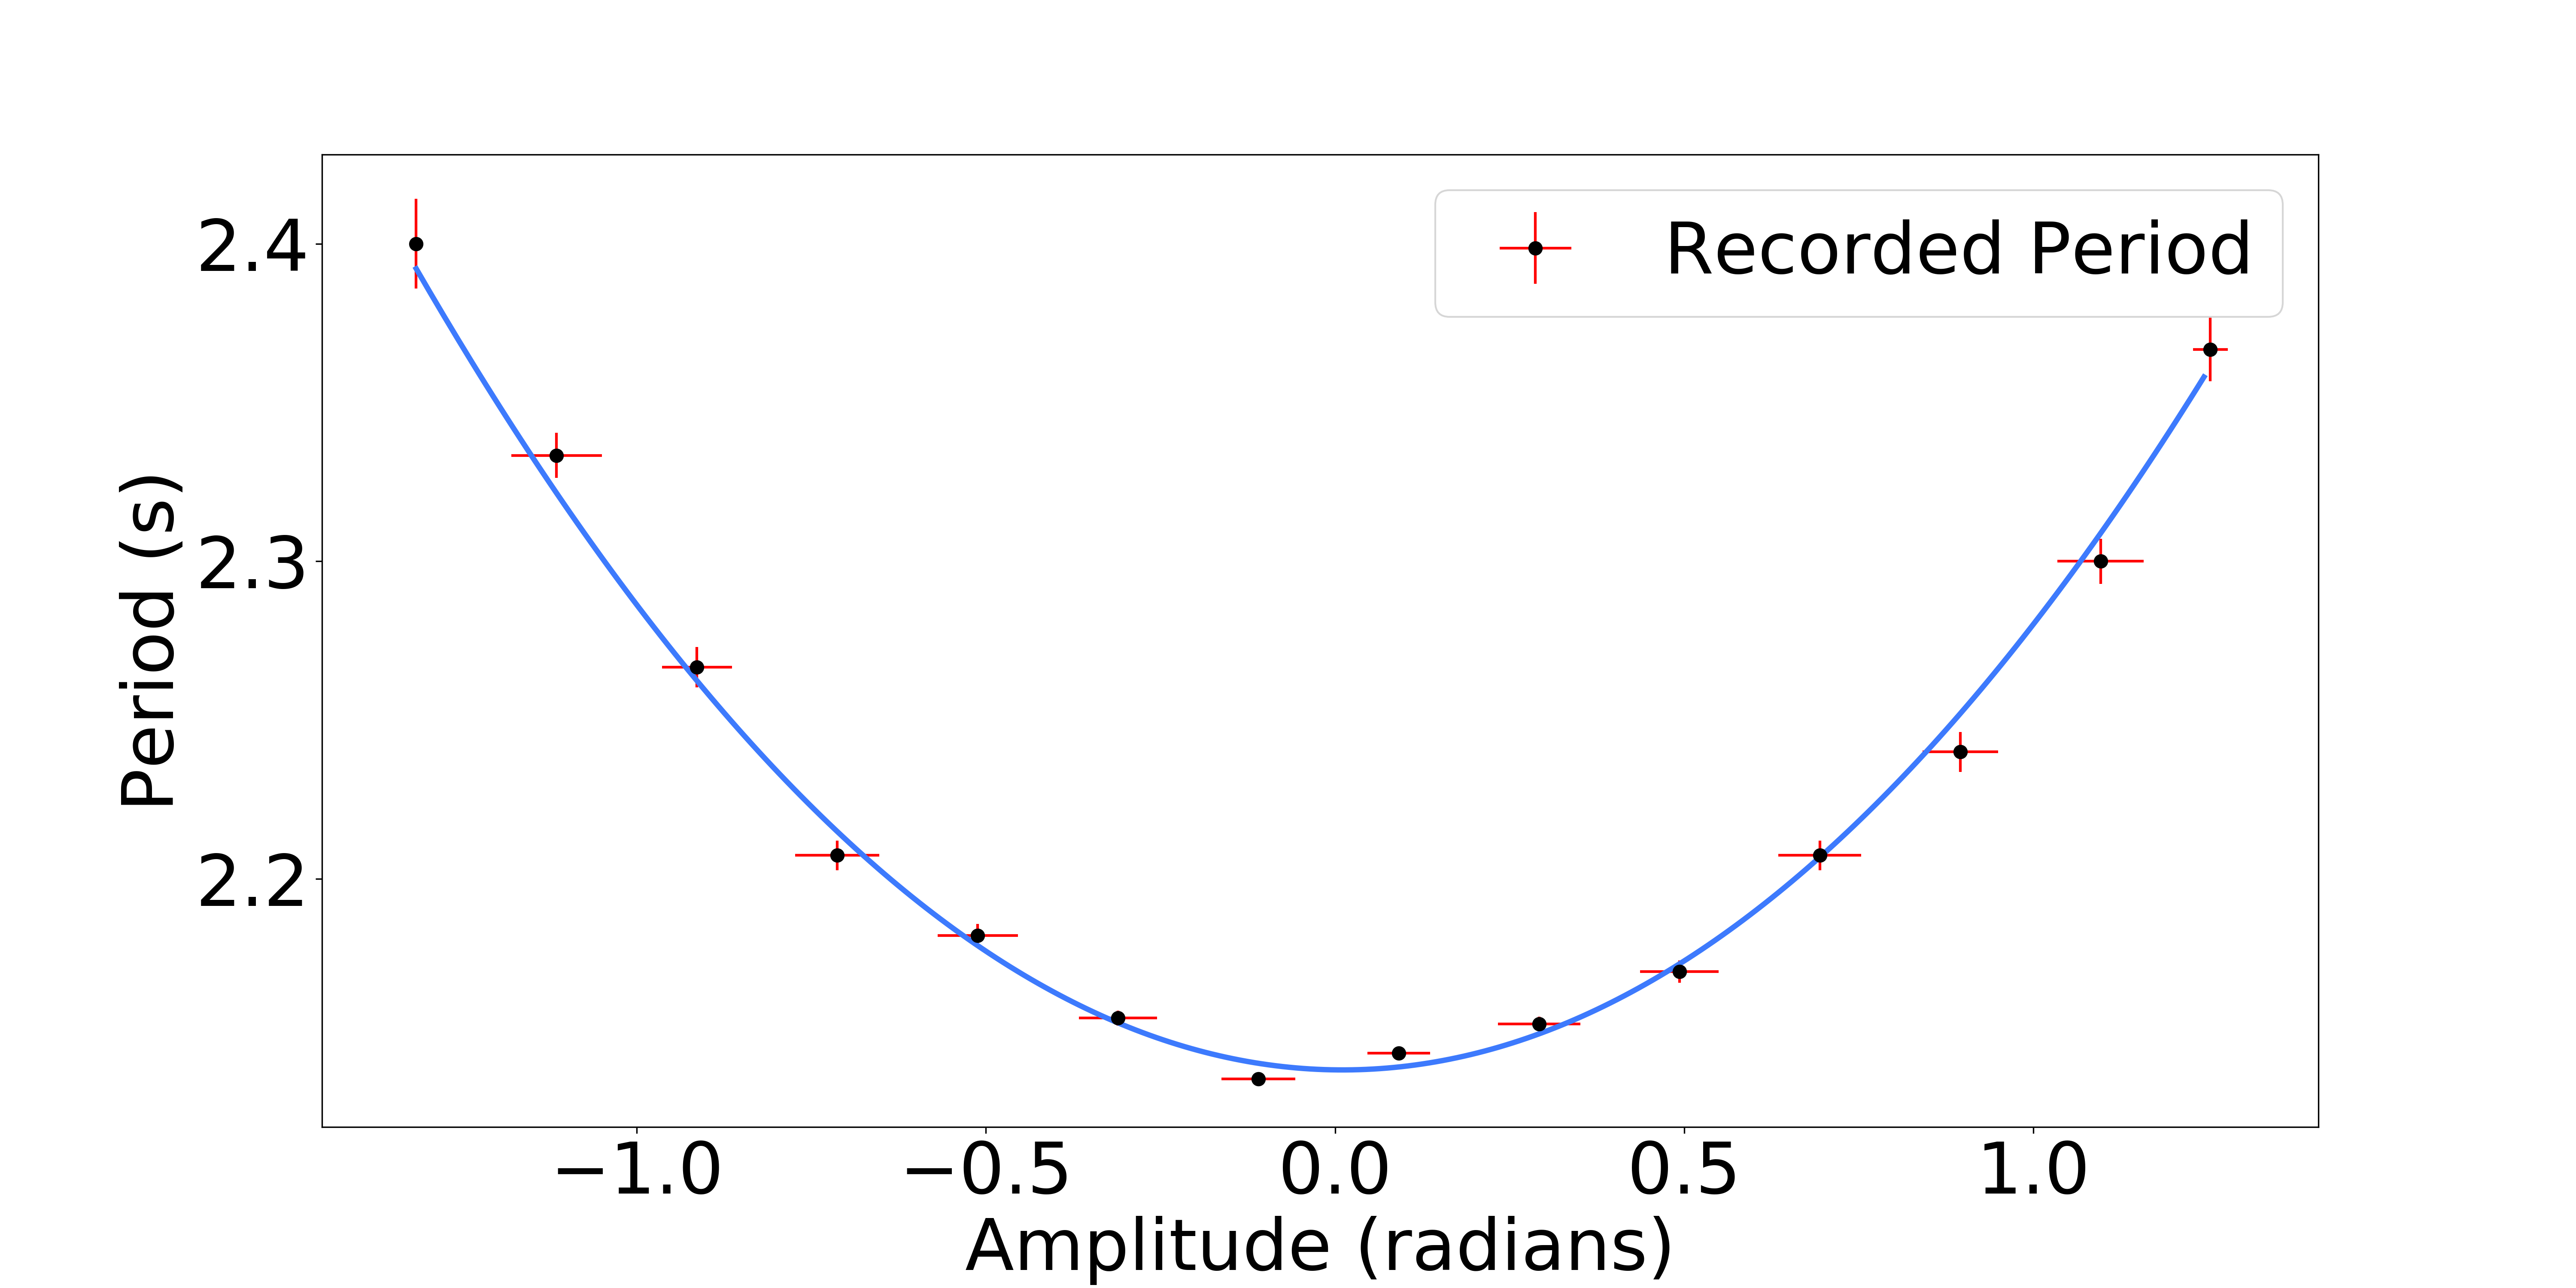
\includegraphics[width=\linewidth]{Figures/period-vs-amplitude.png}

    \caption{A plot of the period as a function of the amplitude. Note that the amplitude ranges from negative (to the left of the pivot) and positive (to the right), in order to test for asymmetry.}
    \label{fig:period-vs-amplitude}
\end{figure}
As a result, we can perform a linear regression by plotting the period against the square of the amplitude, as shown in figure \ref{fig:period-vs-amplitude-linear}. Using this linear regression, we verify that the period is $T_0=2.140 \pm 0.005$ and $\beta = 0.0670 \pm 0.0007$, as shown by considering a full quadratic fit. This confirms that the pendulum is exhibiting a very symmetric motion.
\begin{figure}[!h]
    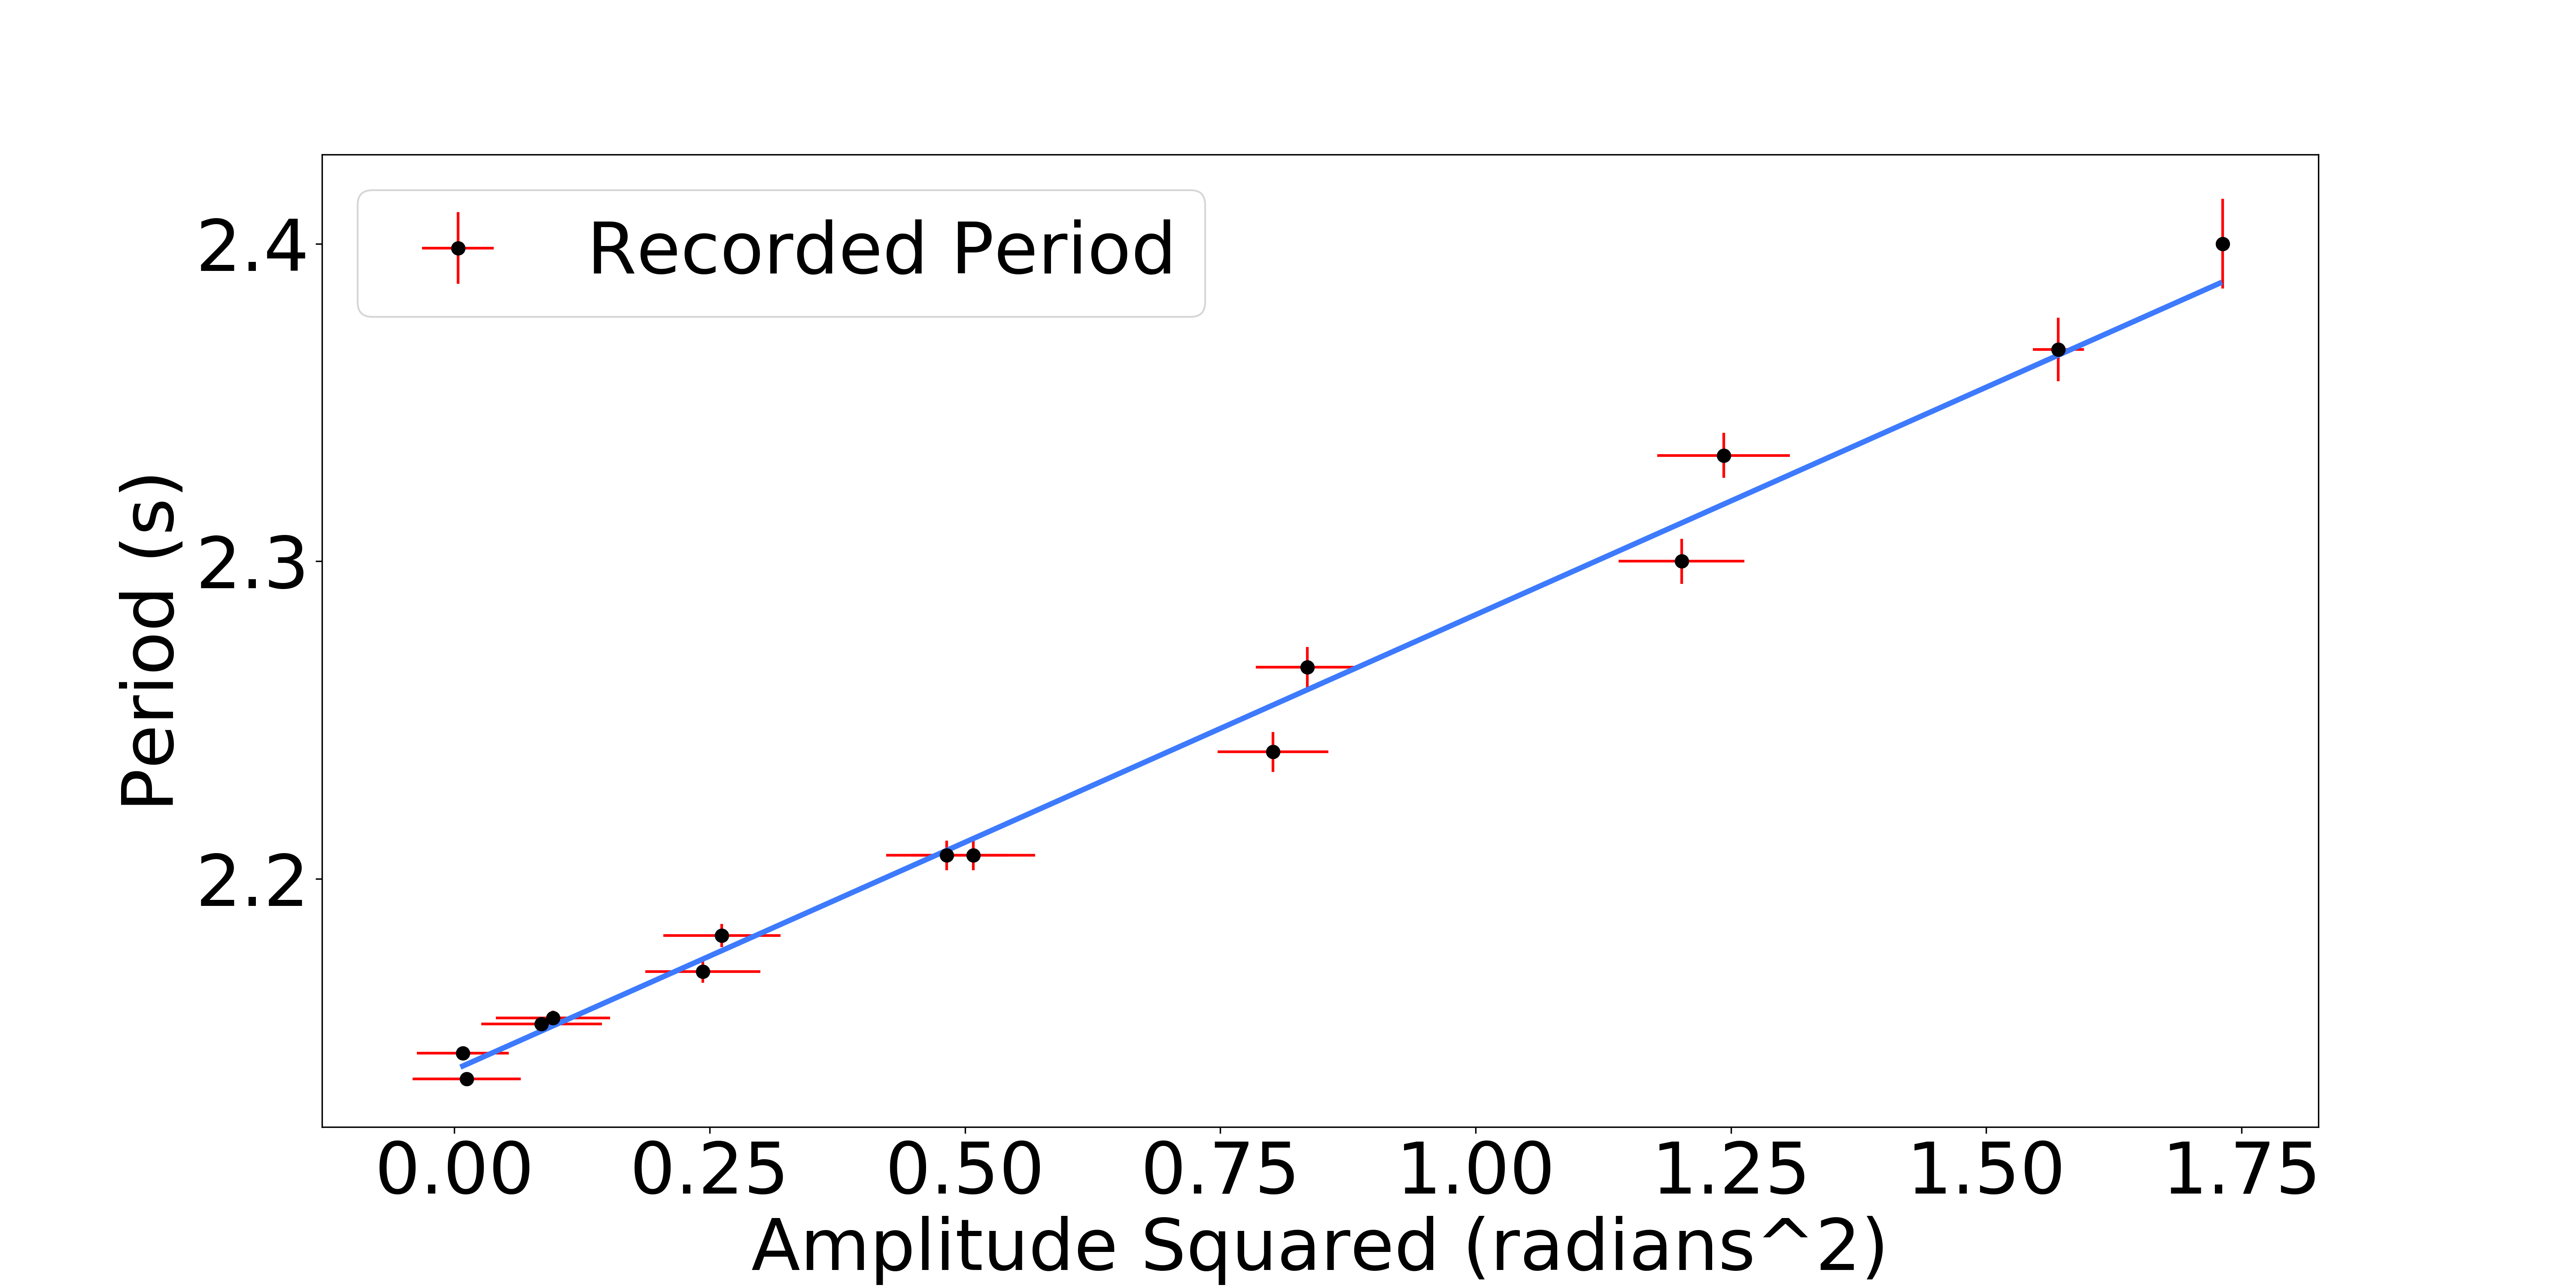
\includegraphics[width=\linewidth]{Figures/period-vs-amplitude-linear.png}

    \caption{A plot of the period as a function of the square of the amplitude. Similar value for $T_0$ and $\beta$ was obtained. The quality of the fit is given by $R^2=0.99$.}
    \label{fig:period-vs-amplitude-linear}
\end{figure}
\subsection{Q Factor}
Over $100,000$ frames were analyzed using the software \textit{Tracker}. There were hundreds of oscillations and it would not be meaningful to plot everything in one figure. Instead, the first $45$ seconds are plotted in figure \ref{fig:intervals}.
\begin{figure}[!h]
    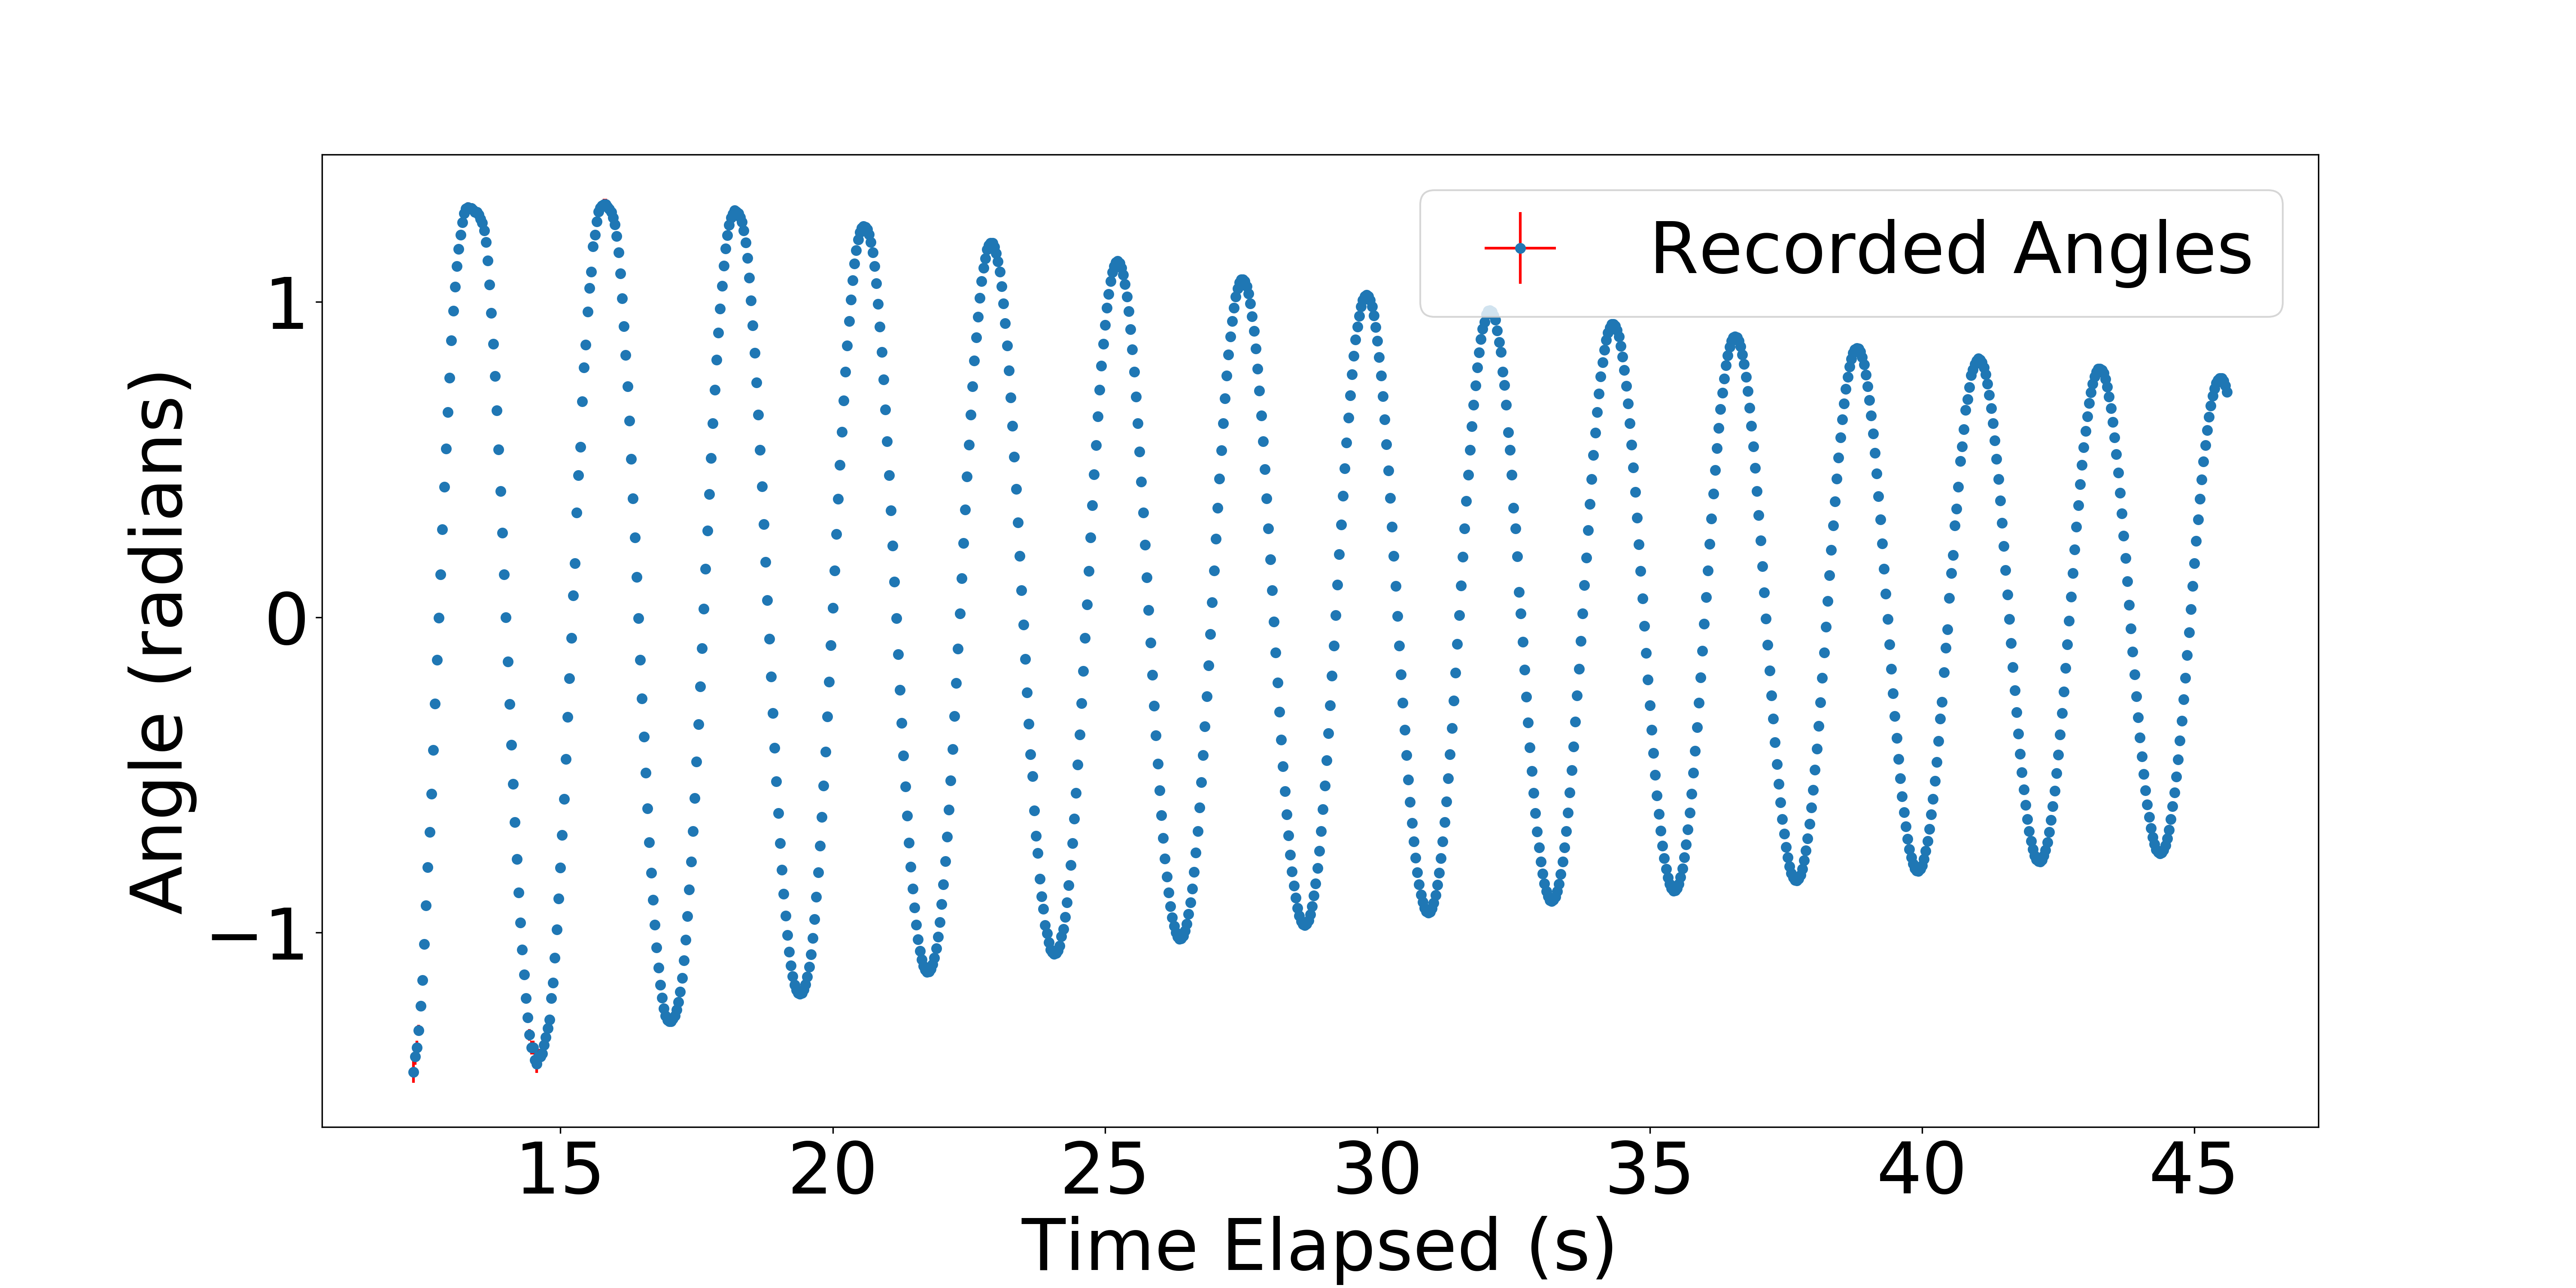
\includegraphics[width=\linewidth]{figures/first-1000.png}

    \caption{A few selected data points. The red lines represent the error bars. Notice that qualitatively, the curve resembles that of a decaying exponential.}
    \label{fig:intervals}
\end{figure}
If the amplitudes follow the predicted envelope function, then plotting their natural logarithms should yield a straight line:
\begin{equation}
    \ln(\theta)=\ln(\theta_0)-\frac{t}{\tau}
    \label{eq:}
\end{equation}
where the negative inverse of the slope gives the time constant $\tau$, as shown in figure \ref{fig:period-vs-amplitude}. If we were to use this plot, then the time constant is given as $\tau = 147.8 \pm 0.9 \si{\second}$ and an initial angle of $\theta_0=37.4 \pm 0.5\si{\degree}$.
\begin{figure}[!h]
    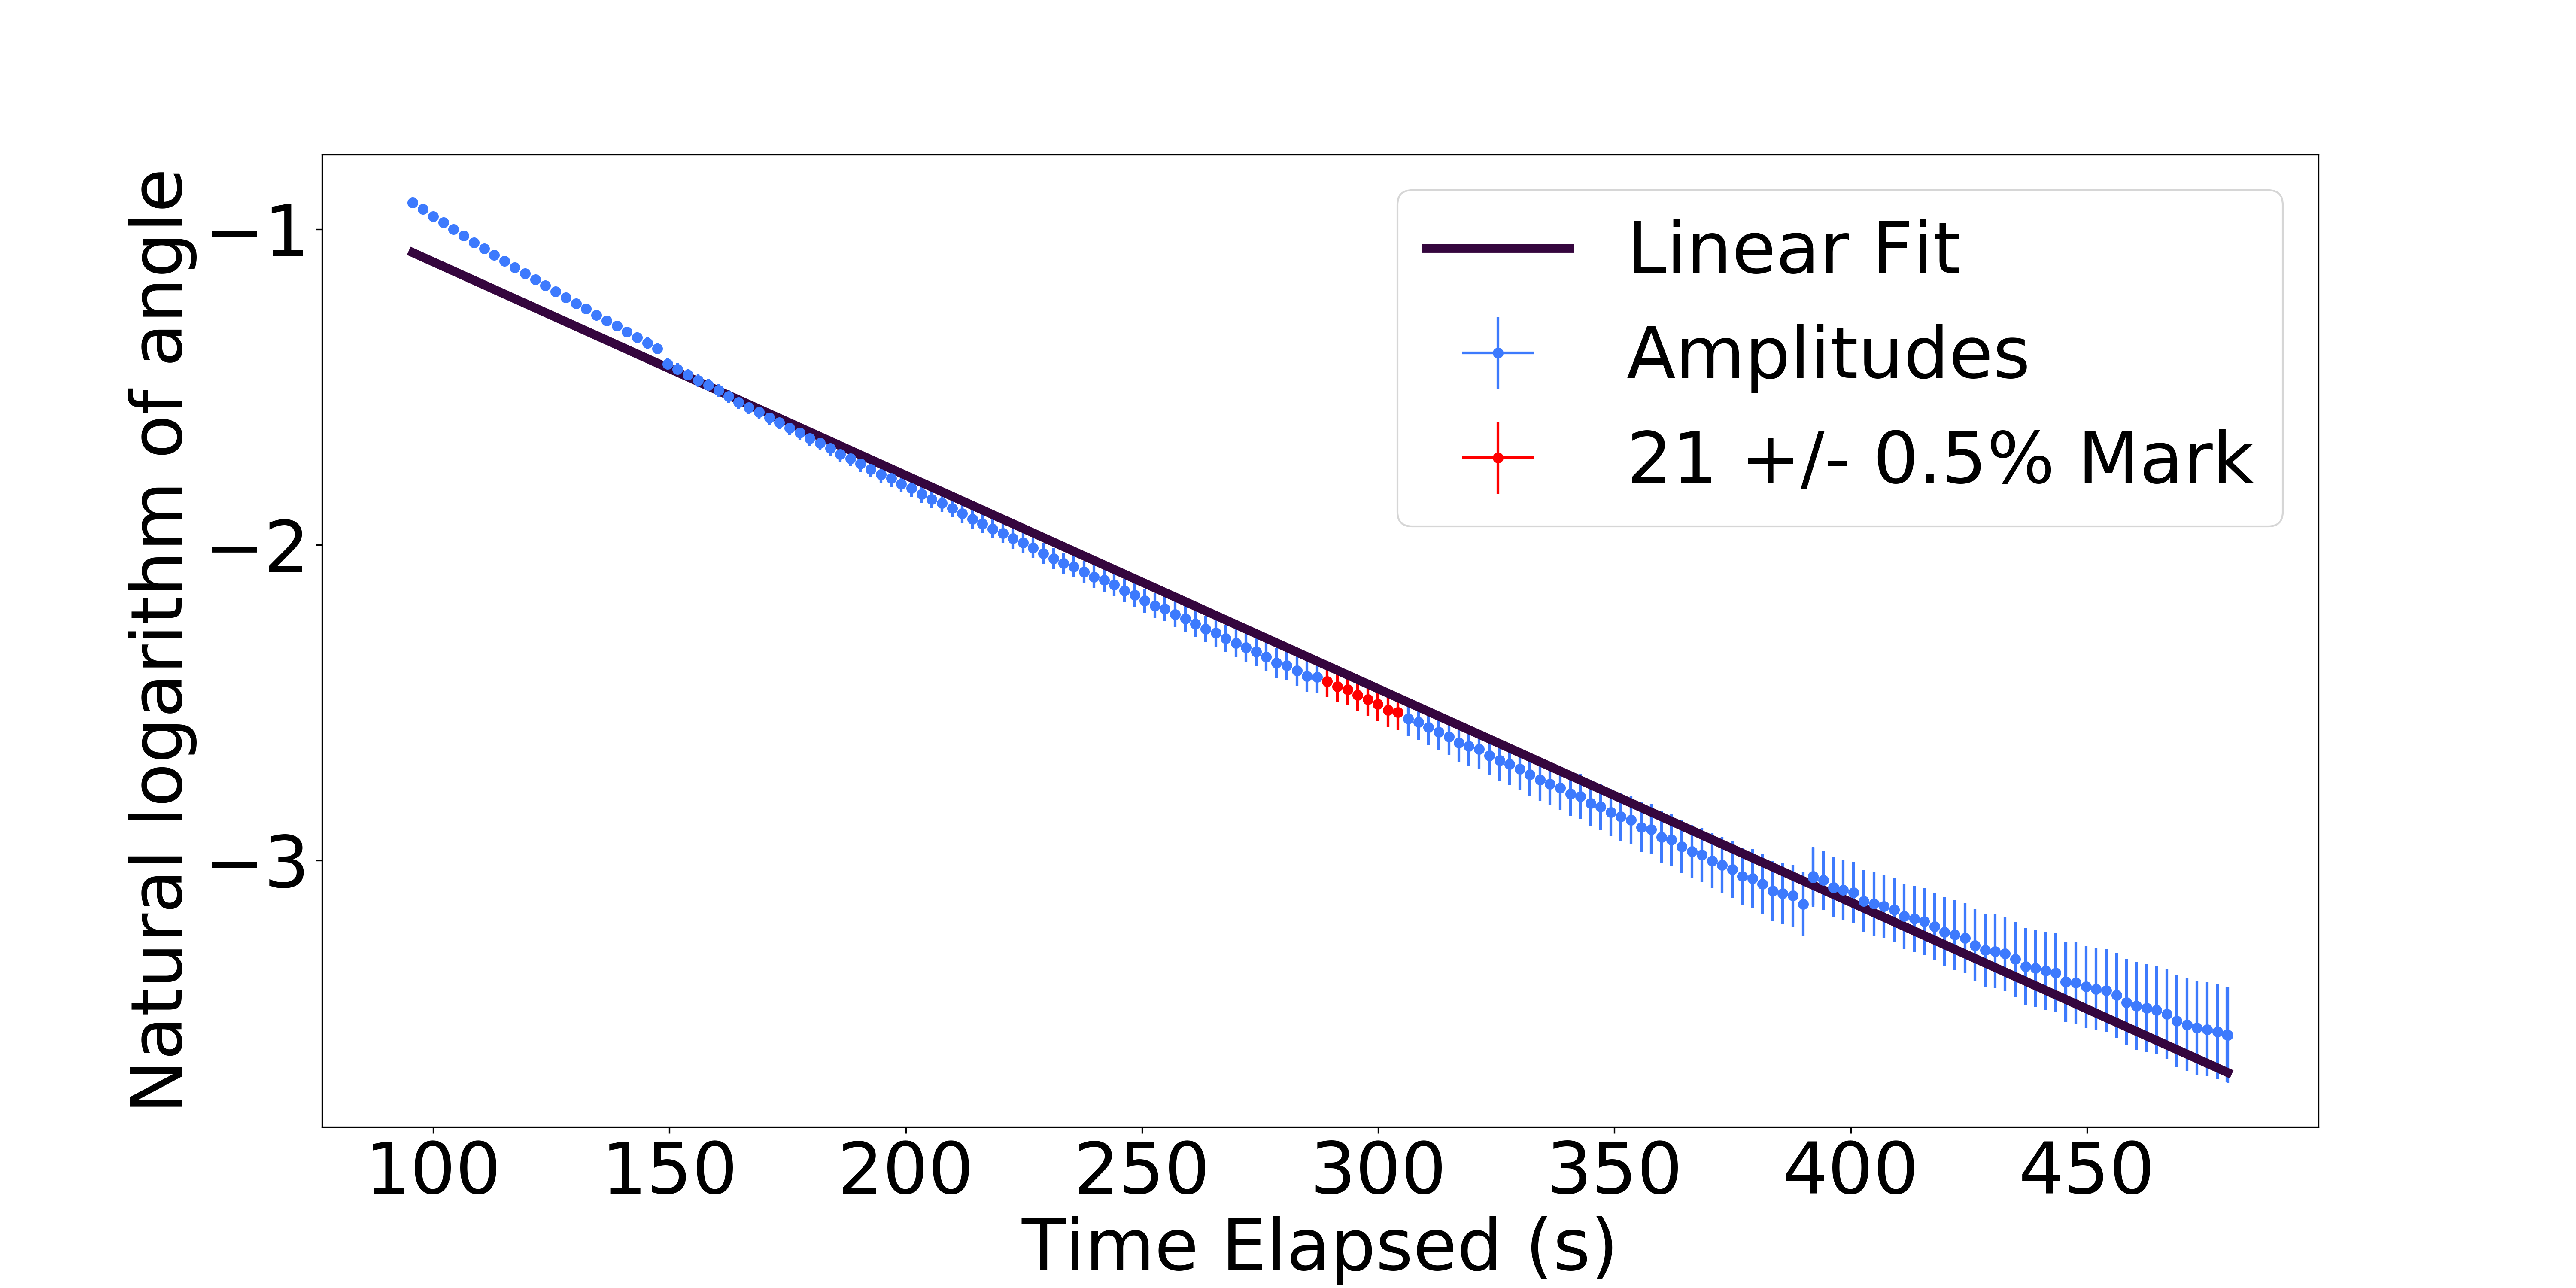
\includegraphics[width=\linewidth]{figures/amplitude-vs-time-fitted.png}

    \caption{A plot of the natural log of the amplitudes with the line of best fit. The desired linear pattern was not seen. The quality of the fit is given by $R^2=0.99$. The red dots denote the amplitudes which fall within $21 \pm 0.5\%$ of the initial amplitude.}
    \label{fig:amplitude-vs-time}
\end{figure}
In the angle dependance section, the period was measured to be  $T=2.140 \pm 0.005 \si{\second}$. This gives the first $Q$ value of $Q=217\pm 1$ by numerically fitting the plot. Using the second method of counting the number of oscillations, I get $Q=277 \pm 3$ by considering the first and last data point that is within $0.5\%$ to $21\%$ and finding the average. In the discussion section, I claim that these represent the lower and upper bounds respectively, so a reasonable estimate for the $Q$ factor would be:
\begin{equation}
    Q_\text{est} = 250 \pm 30
    \label{eq:}
\end{equation}
using Python, since we are not supposed to use proper error propagation techniques yet. In general, a high $Q$ factor is preferred, since the deviation in the amplitude over a given period is smaller. In future experiments, I will investigate how the initial angle may impact the period of oscillation, and being able to maintain near a certain amplitude will make period measurements more accurate.

The dispecrancy between these two $Q$ values can come from an incorrect model, which will be looked at thoroughly in the discussion.

\subsection{Length Dependance}
I will linearize the data in two different ways: first by plotting the square of the period $T^2$ against the length of the string $\ell$ as seen in figure \ref{fig:linear-1}. This is done in order to determine relevant coefficients and determine the center of mass. Then I will plot $\log(\ell_\text{cm}+\Delta L)$ against $\log(T)$ to determine that the relationship is a square root model, which is shown in figure \ref{fig:log-2}.
\begin{figure}[!h]
    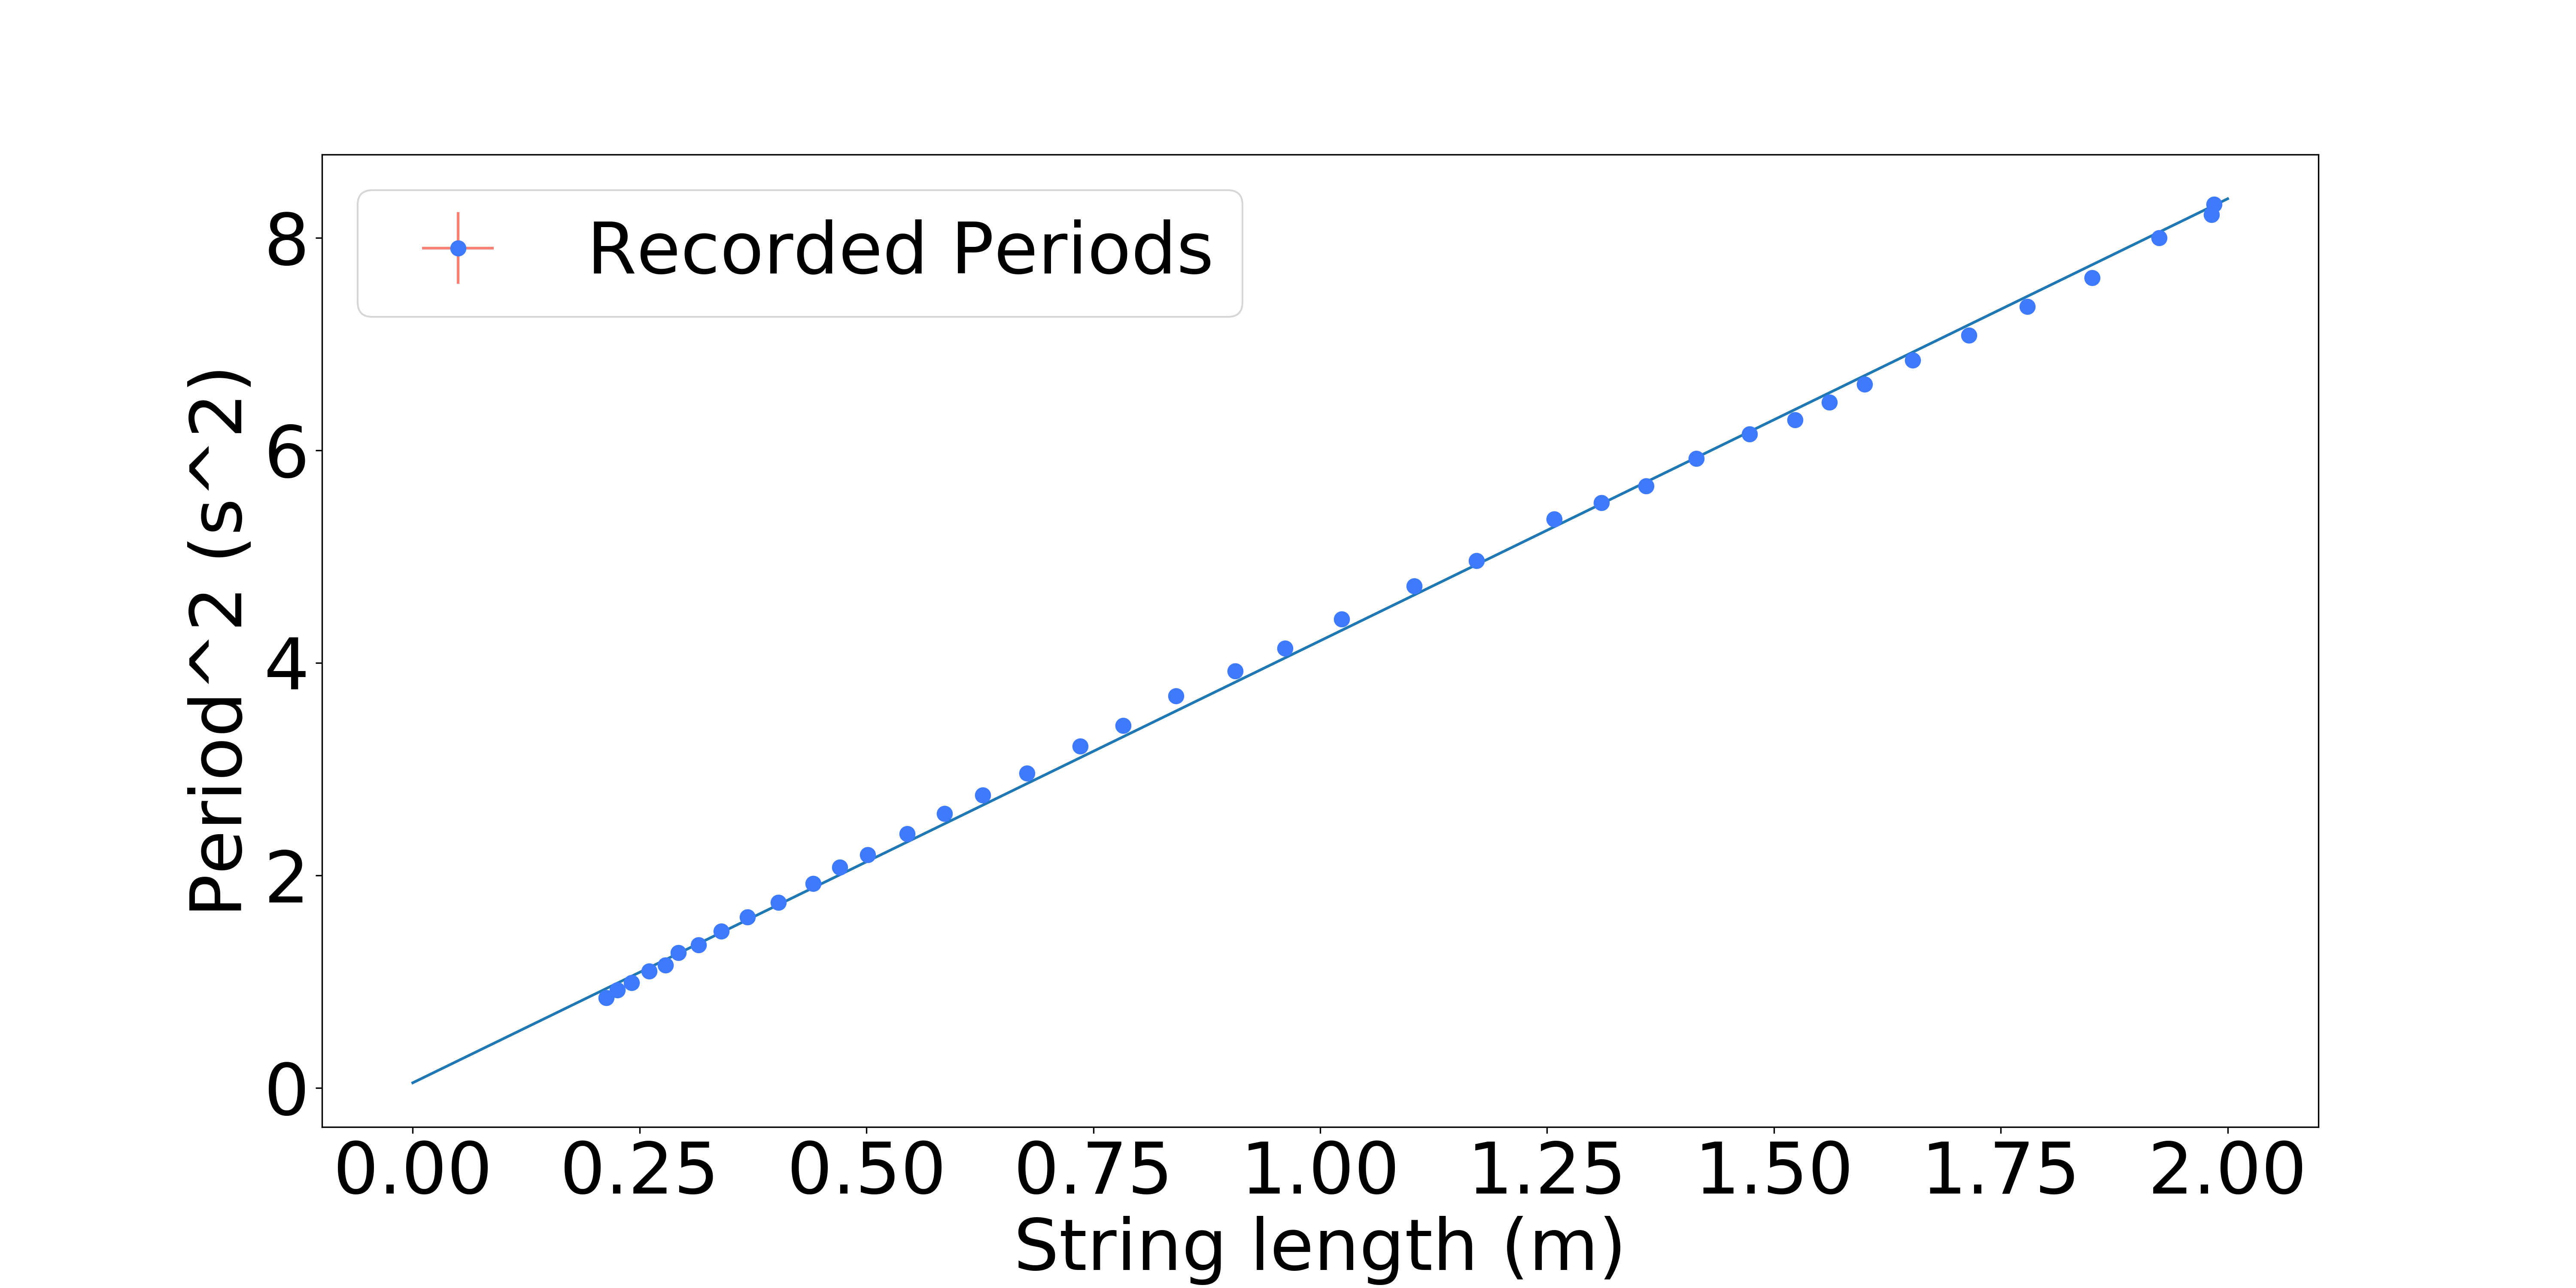
\includegraphics[width=\linewidth]{Figures/linear_1.png}
    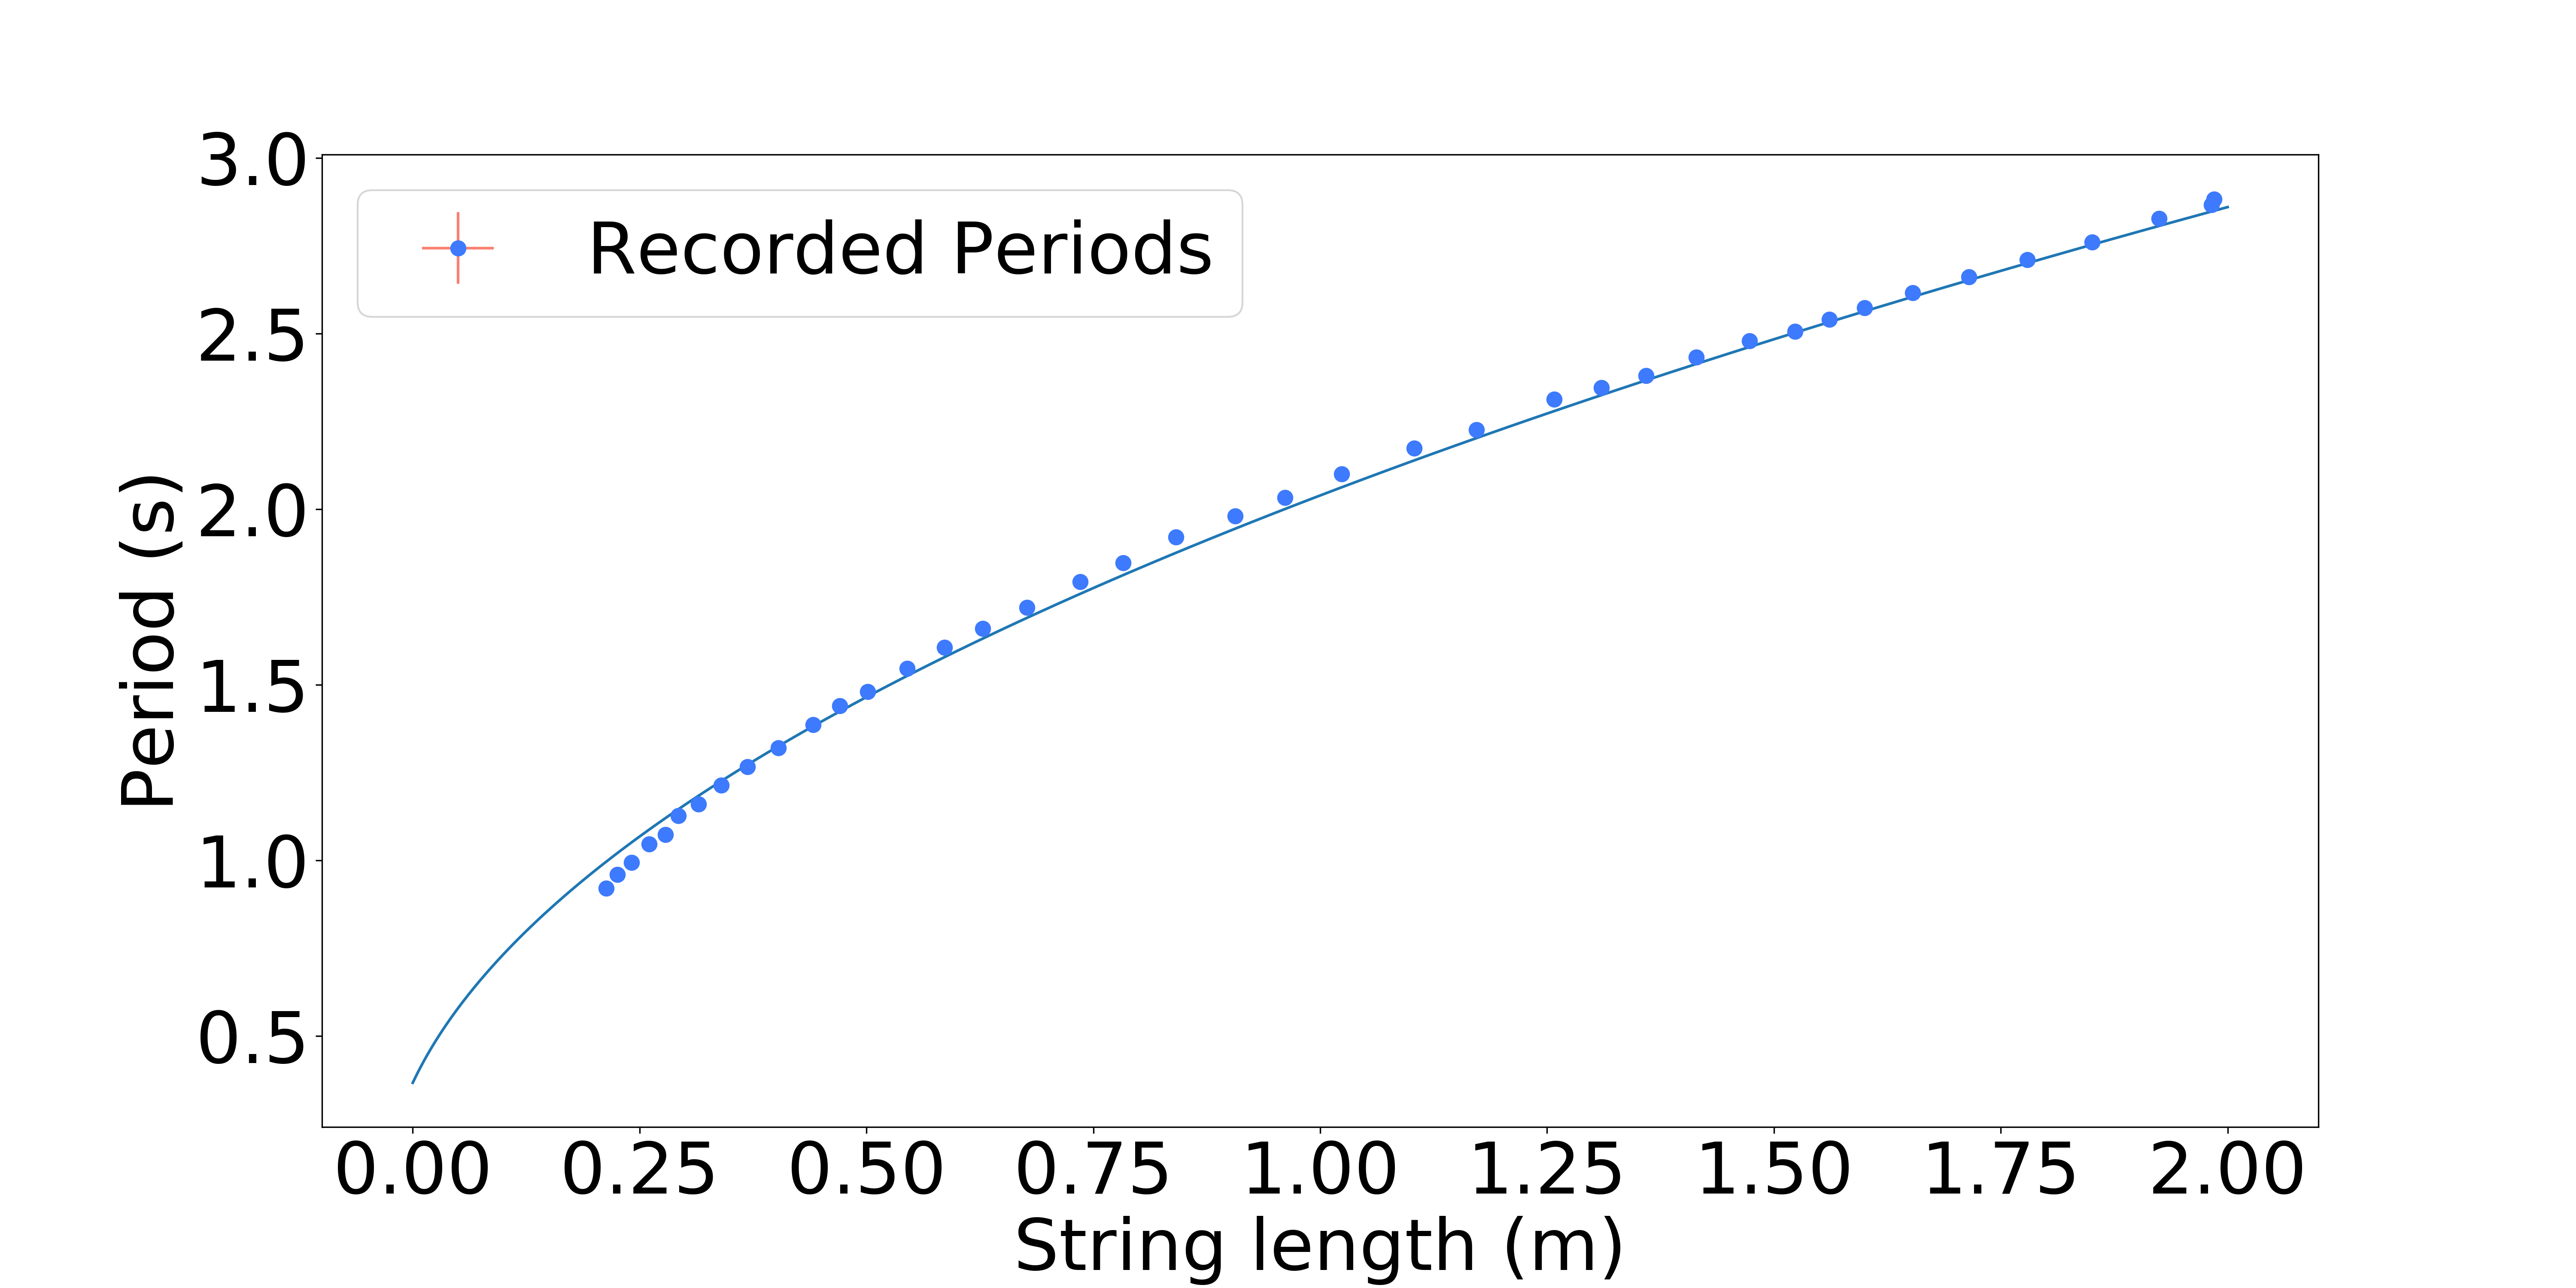
\includegraphics[width=\linewidth]{Figures/normal_1.png}

    \caption{Above: A plot of the square of the period against the length of the string. Below: A plot of only the period against the length of the rope. Note that the fitted curve overestimates the period for short string lengths.}
    \label{fig:linear-1}
\end{figure}
For the linearization, the slope $m$ and intercept $b$ are given by:
\begin{align}
    m &= 4.16 \pm 0.02 \si{\second\squared\per\meter} \\ 
    b &= 0.05 \pm 0.02 \si{\second\squared}
\end{align}
However, since the formula $T = 2\pi\sqrt{\frac{\ell_\text{cm}}{g}}$ is not accurate when the string length is comparable in size to the length of the water bottle, the two curves plotted in figure \ref{fig:linear-1} are not representative of the true curve. Instead, it may be better to only plot the half of the data which use a larger string length, as shown in figure \ref{fig:plot-2}
\begin{figure}[!h]
    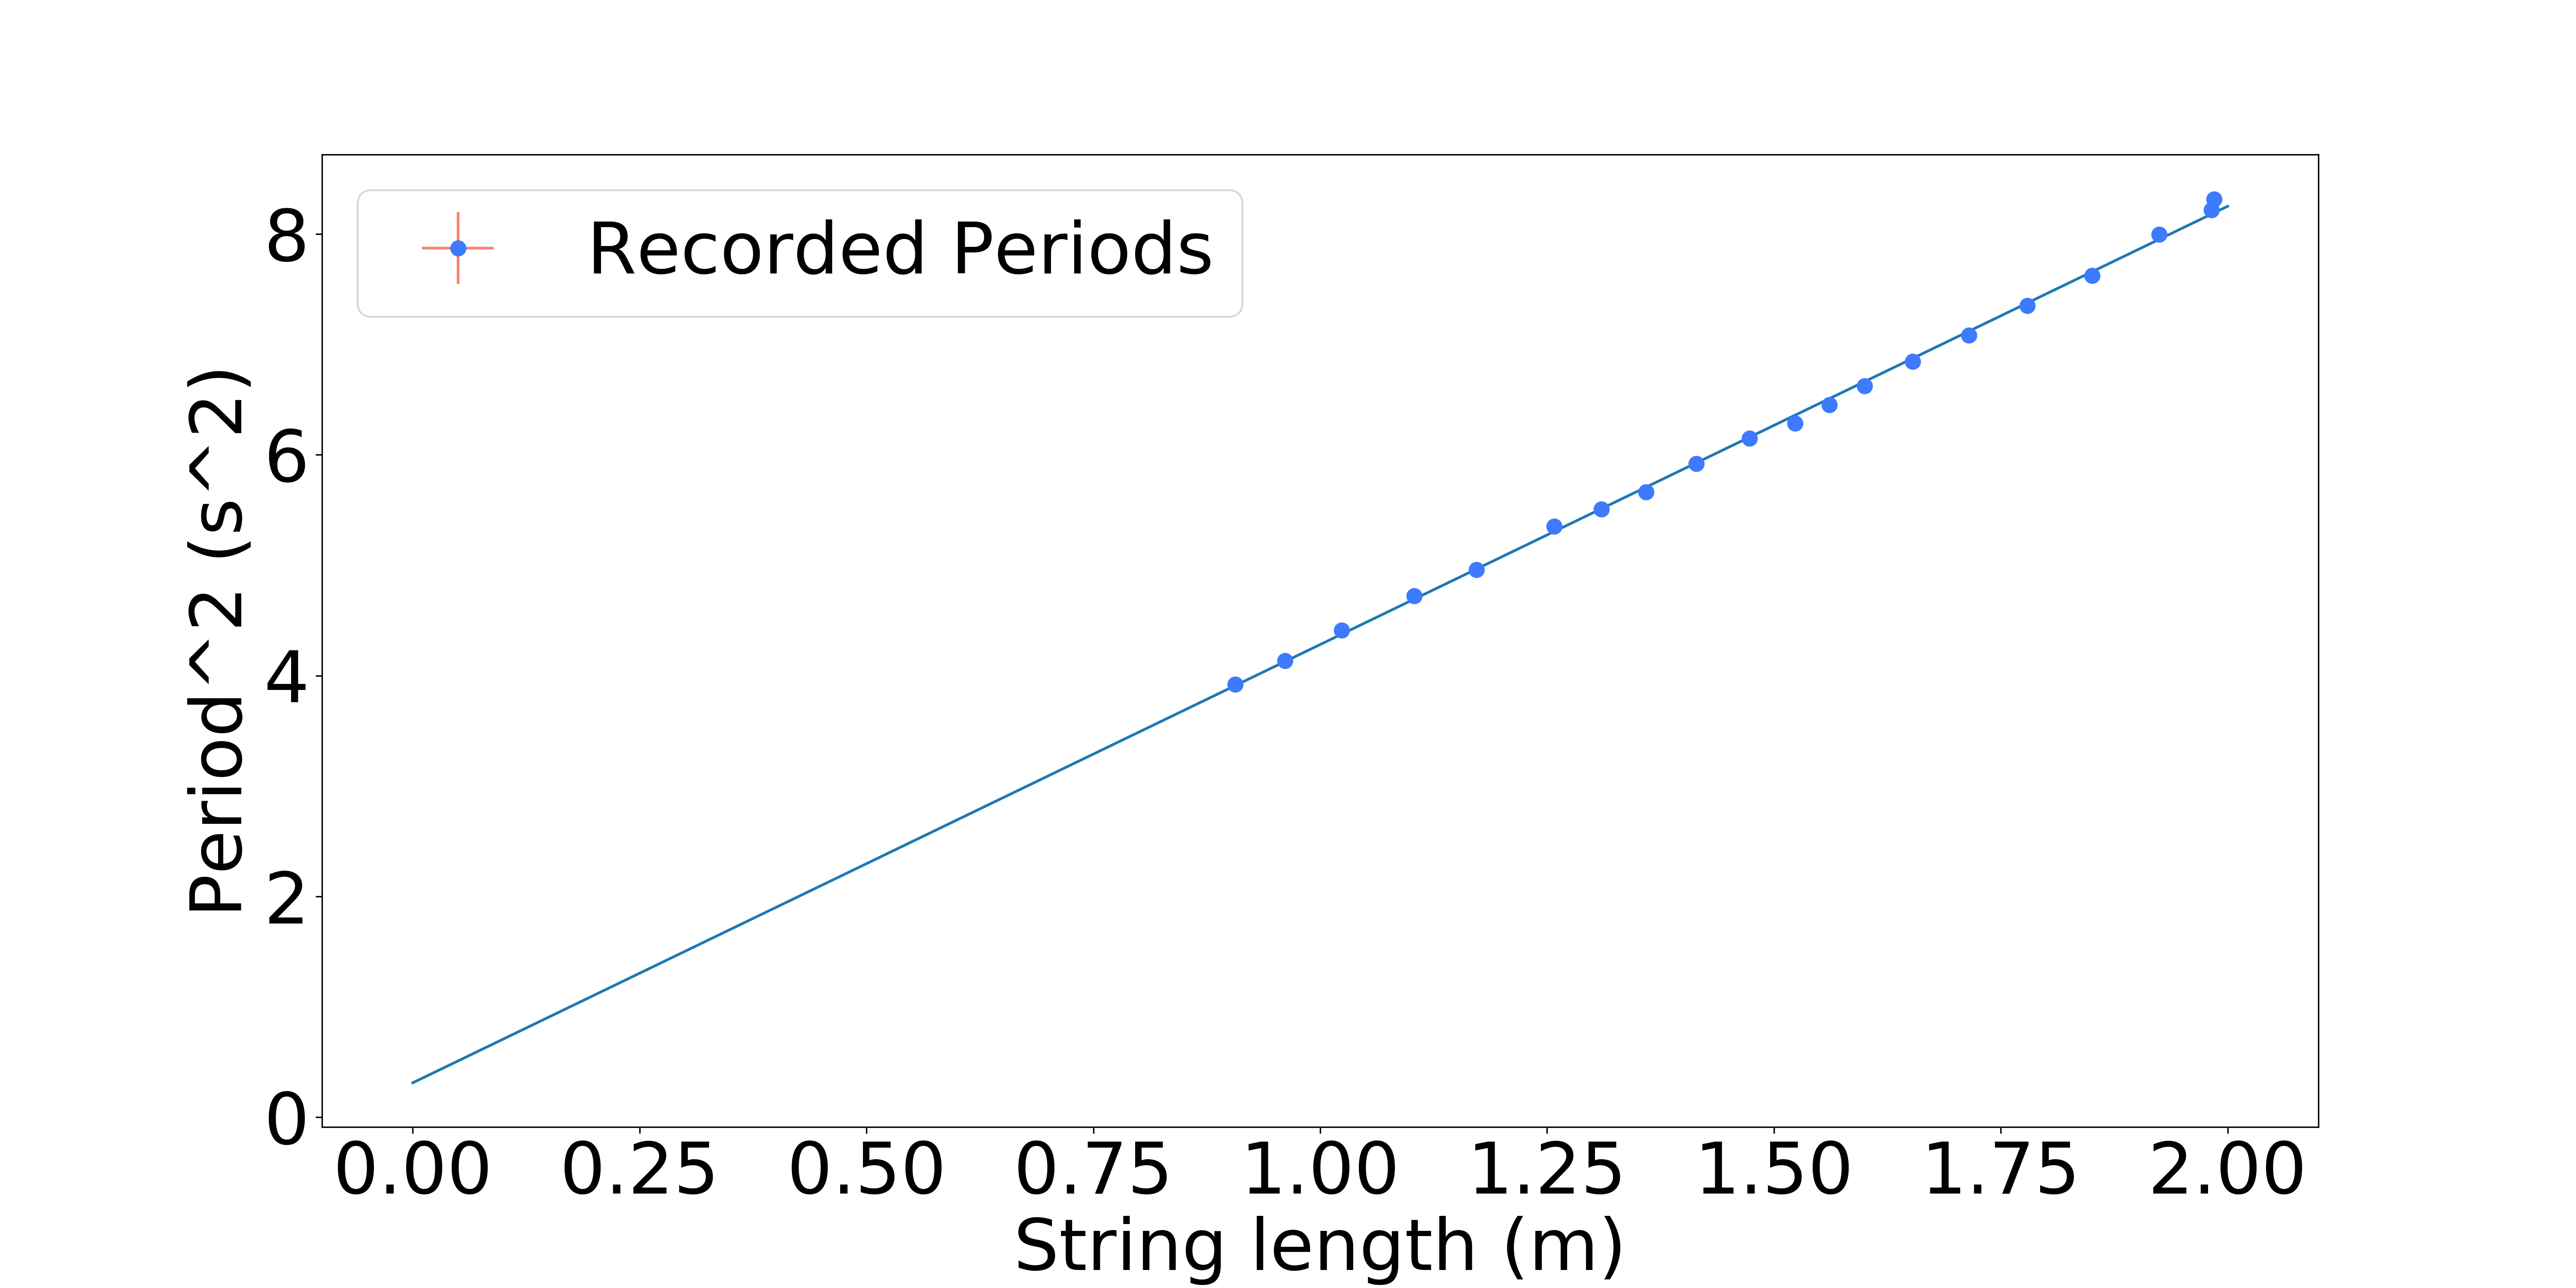
\includegraphics[width=\linewidth]{Figures/linear_2.png}
    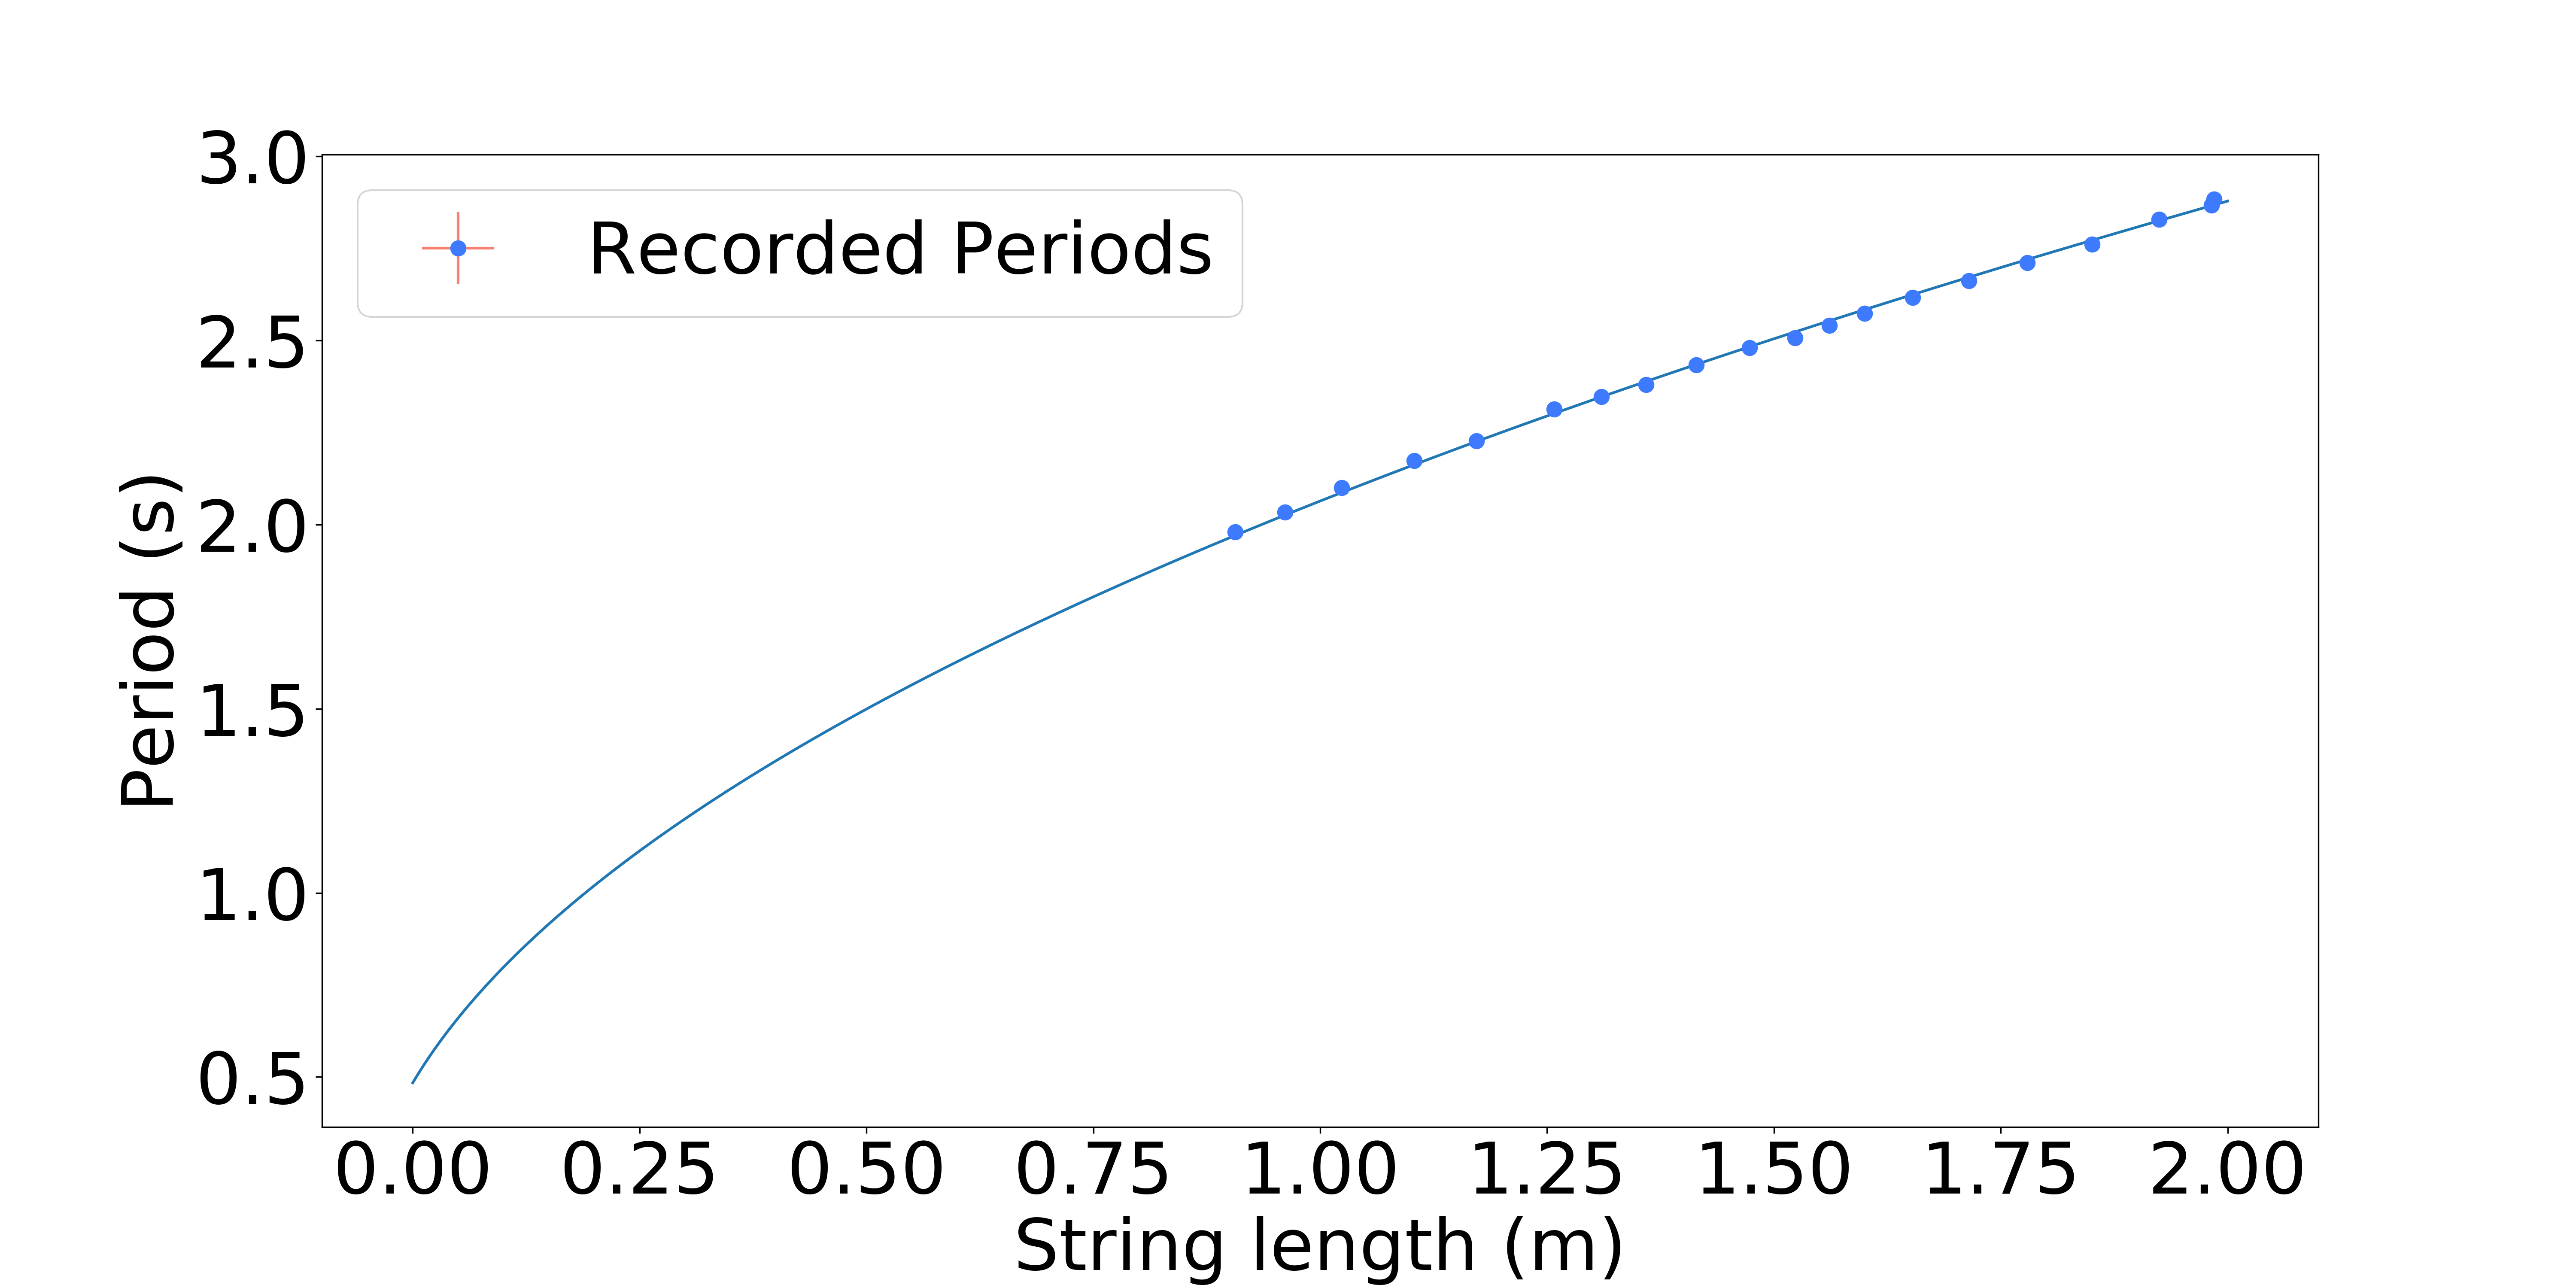
\includegraphics[width=\linewidth]{Figures/normal_2.png}

    \caption{A plot of the period against the length of the string, both linearized (above) and the original (below). Only half the data points were graphed this time to keep the string length high.}
    \label{fig:plot-2}
\end{figure}
This linearization has a slope and intercept of:
\begin{align}
    m &= 3.97 \pm 0.03 \si{\second\squared\per\meter} \\ 
    b &= 0.31 \pm 0.04 \si{\second\squared}
    \label{eq:}
\end{align}
By only looking at trials where a long string was used, the data agrees with the theoretical prediction:
\begin{equation}
    T^2 = \frac{4\pi^2}{g}\left(\ell+\Delta L\right)
    \label{eq:}
\end{equation}
where the theoretical slope is
\begin{equation}
    m_\text{theory} = \frac{4\pi^2}{9.8\pm 0.05} = 4.03 \pm 0.02 \si{\second\squared\per\meter}.
    \label{eq:mtheory}
\end{equation}
This means that the distance from the end of the string to the center of mass is:
\begin{equation}
    \Delta \ell = 0.08 \pm 0.01\si{\meter} 
    \label{eq:}
\end{equation}
We can use this information to make sense of the original value for the slope if we were to look at all data. From equation \ref{eq:proper}, we have:
\begin{equation}
    T^2 = \frac{4\pi^2}{g}\ell \left(1+\frac{\beta d^2}{\ell^2}\right)
\end{equation}
Here, the slope would be dependent on $\ell$, but since the additional factor is greater than one, the slope would always be greater than $\frac{4\pi^2}{g}$, which explains a higher overall slope when the entire data is fitted. We can provide a lower bound for $\beta$ by considering the minimum length $\ell=0.25\si{\meter}$. Since the length of the bottle is $d=0.145 \pm 0.001 \si{\meter}$, we have:
\begin{equation}
    \beta = \frac{0.25^2}{d^2} \cdot \frac{4.16 \pm 0.02}{\left(\frac{4\pi^2}{g}\right)}-1 = 0.09 \pm 0.02
    \label{eq:}
\end{equation}
This is roughly on the order of magnitude of $\beta$ for a uniform cylinder, which is $\beta=\frac{1}{12}$, so the model for small lengths can be considered relatively reasonable. To verify that the power law is $n=\frac{1}{2}$, we can plot the logarithm of the length to the center of mass $\log(\ell_\text{cm})$ with respect to the logarithm of the period $\log(T)$. Therefore, if the relationship between the two were $T = (C\ell_\text{cm})^n$, then the log-log plot would yield
\begin{equation}
    \log(T) = n\left(\log(\ell_\text{cm}) + \log(C)\right)
    \label{eq:}
\end{equation}
giving $n$ as the slope and $n\log(C)$ as the y-intercept. This is shown in figure \ref{fig:log-2}.
\begin{figure}[!h]
    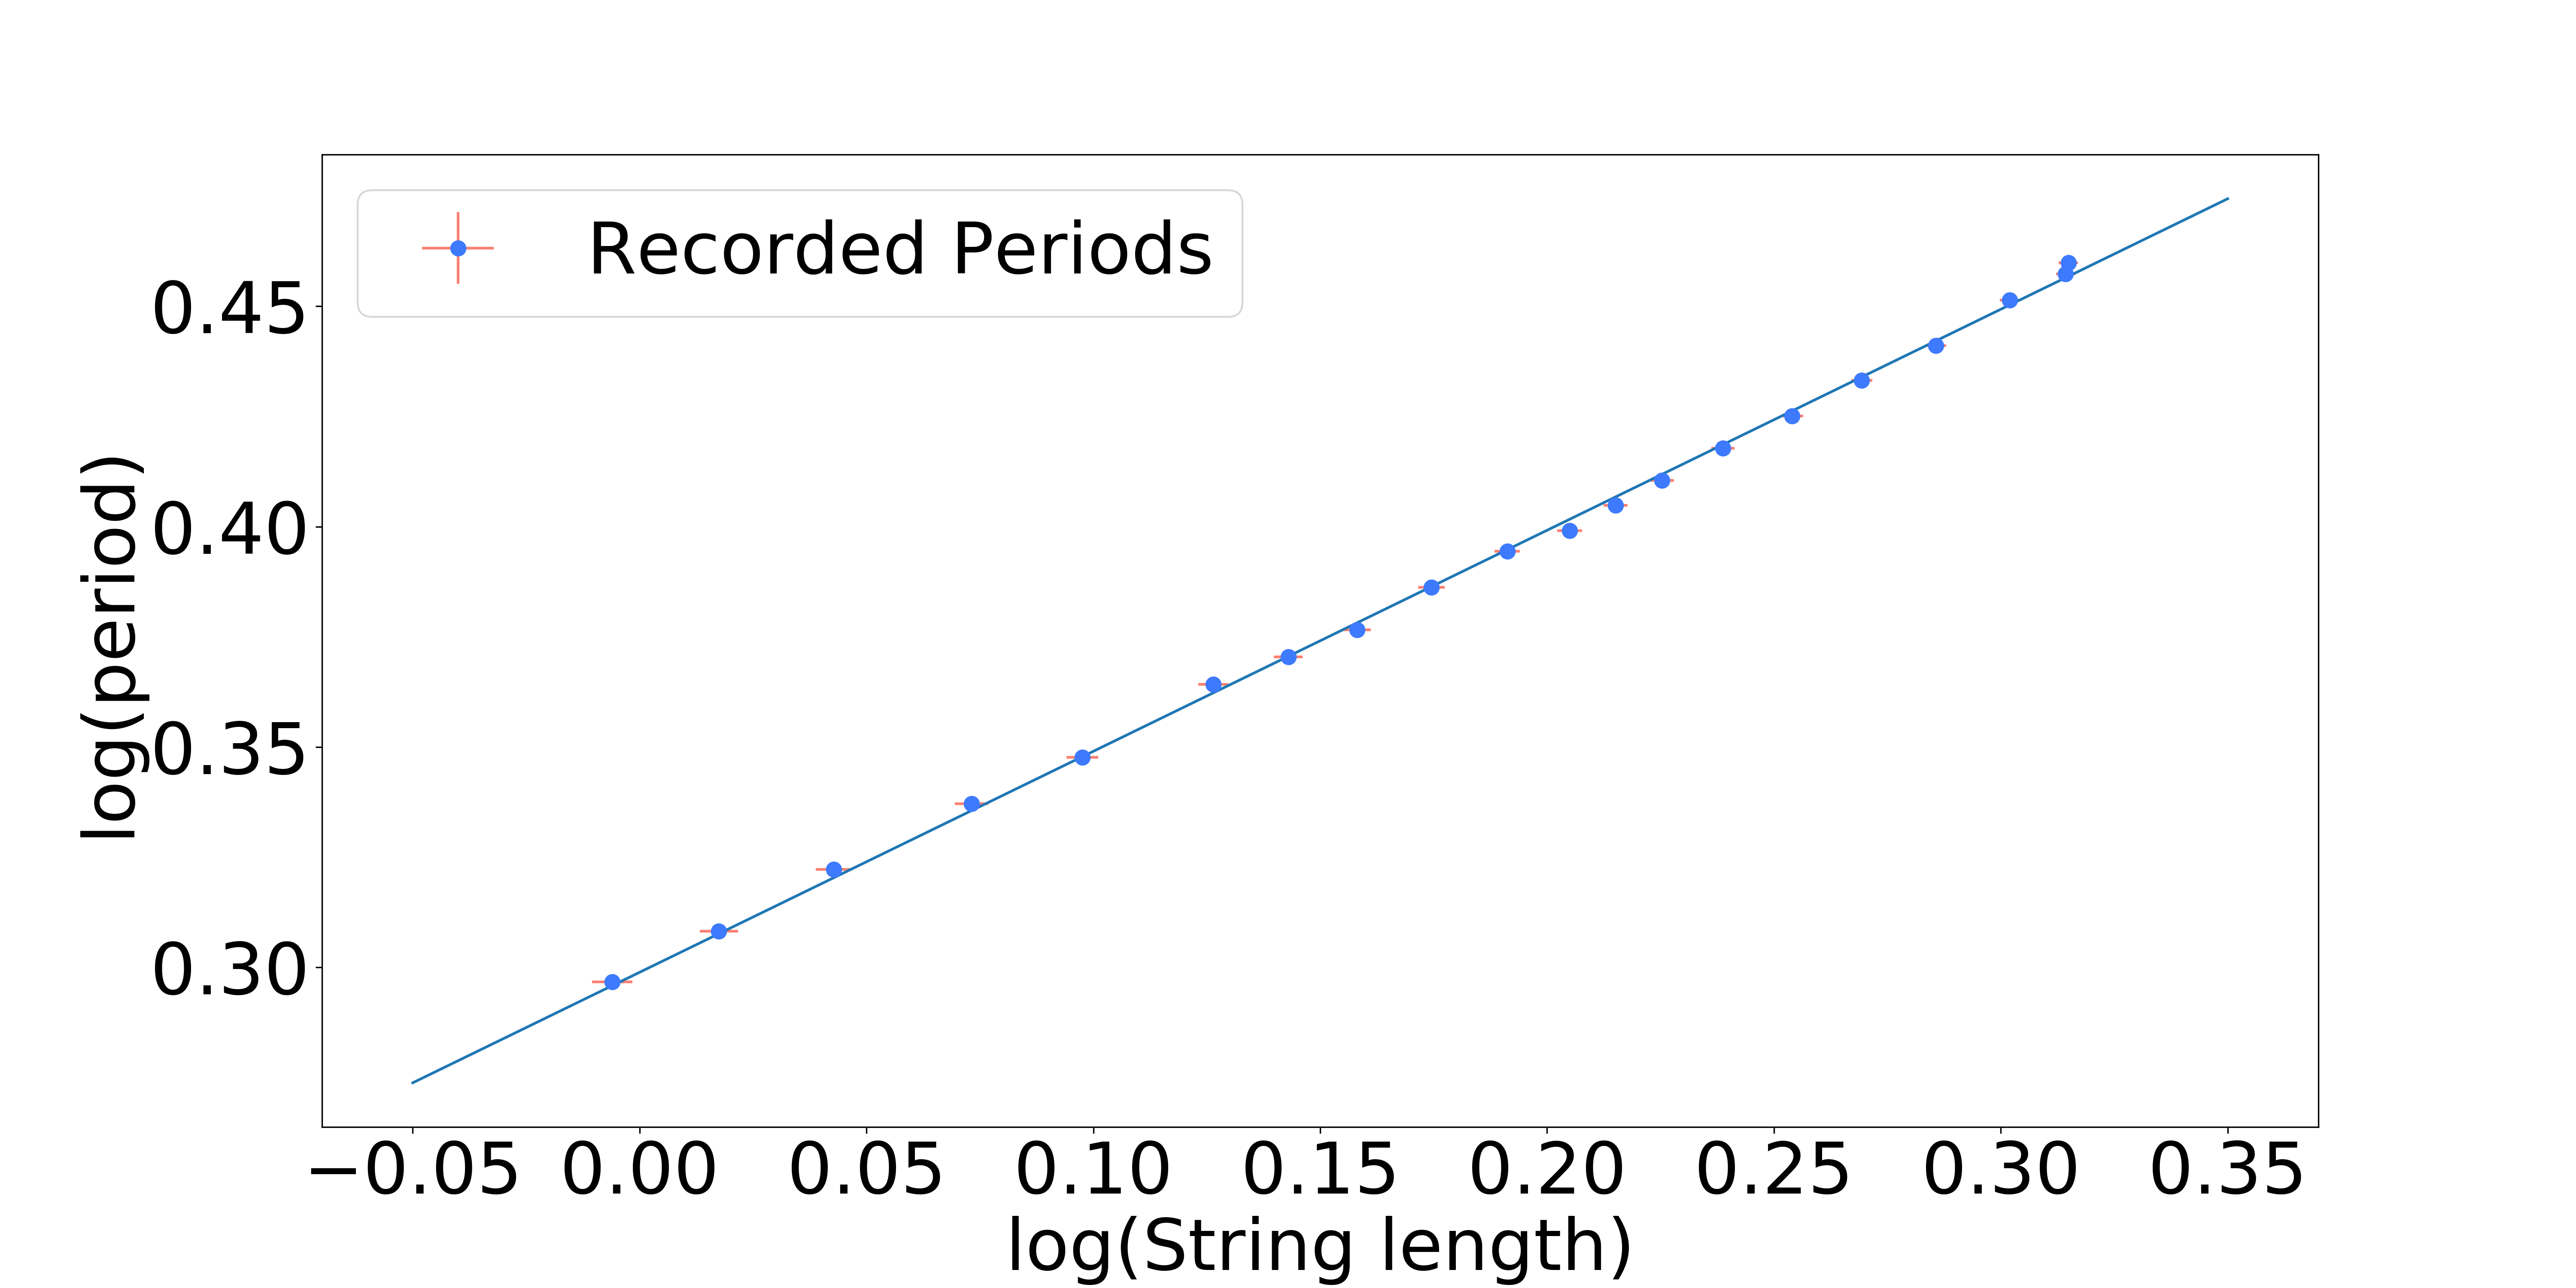
\includegraphics[width=\linewidth]{Figures/log_2.png}

    \caption{A log log plot of the period vs the distance to the center of mass, which was calculated from the previous analysis. Note that only half of the data with large values for length were plotted, in order to ensure that other effects were not important.}
    \label{fig:log-2}
\end{figure}
The slope $m$ and the y-intercept $b$ are:
\begin{align}
    m &= 0.501 \pm 0.004 \\ 
    b &= 0.2989 \pm 0.0009
\end{align}
Here, all units are scaled in such a way that they are dimensionless. Since the power is given by the slope, it agrees with the theoretical model where the relationship between period and length was a square root function. We can also verify that the theoretically predicted $y$ intercept is:
\begin{equation}
    b_\text{theory} = \frac{1}{2}\log\left(\frac{4\pi^2}{g}\right) = 0.303 \pm 0.001
    \label{eq:}
\end{equation}
which roughly agrees with the value obtained from the logarithmic plot.
\subsection{Mass Dependance}
Various masses from $0.029\si{\kilogram}$ to $0.338\si{\kilogram}$ were used for the pendulum, and shown in figure \ref{fig:mass-simple}.
\begin{figure}[!h]
    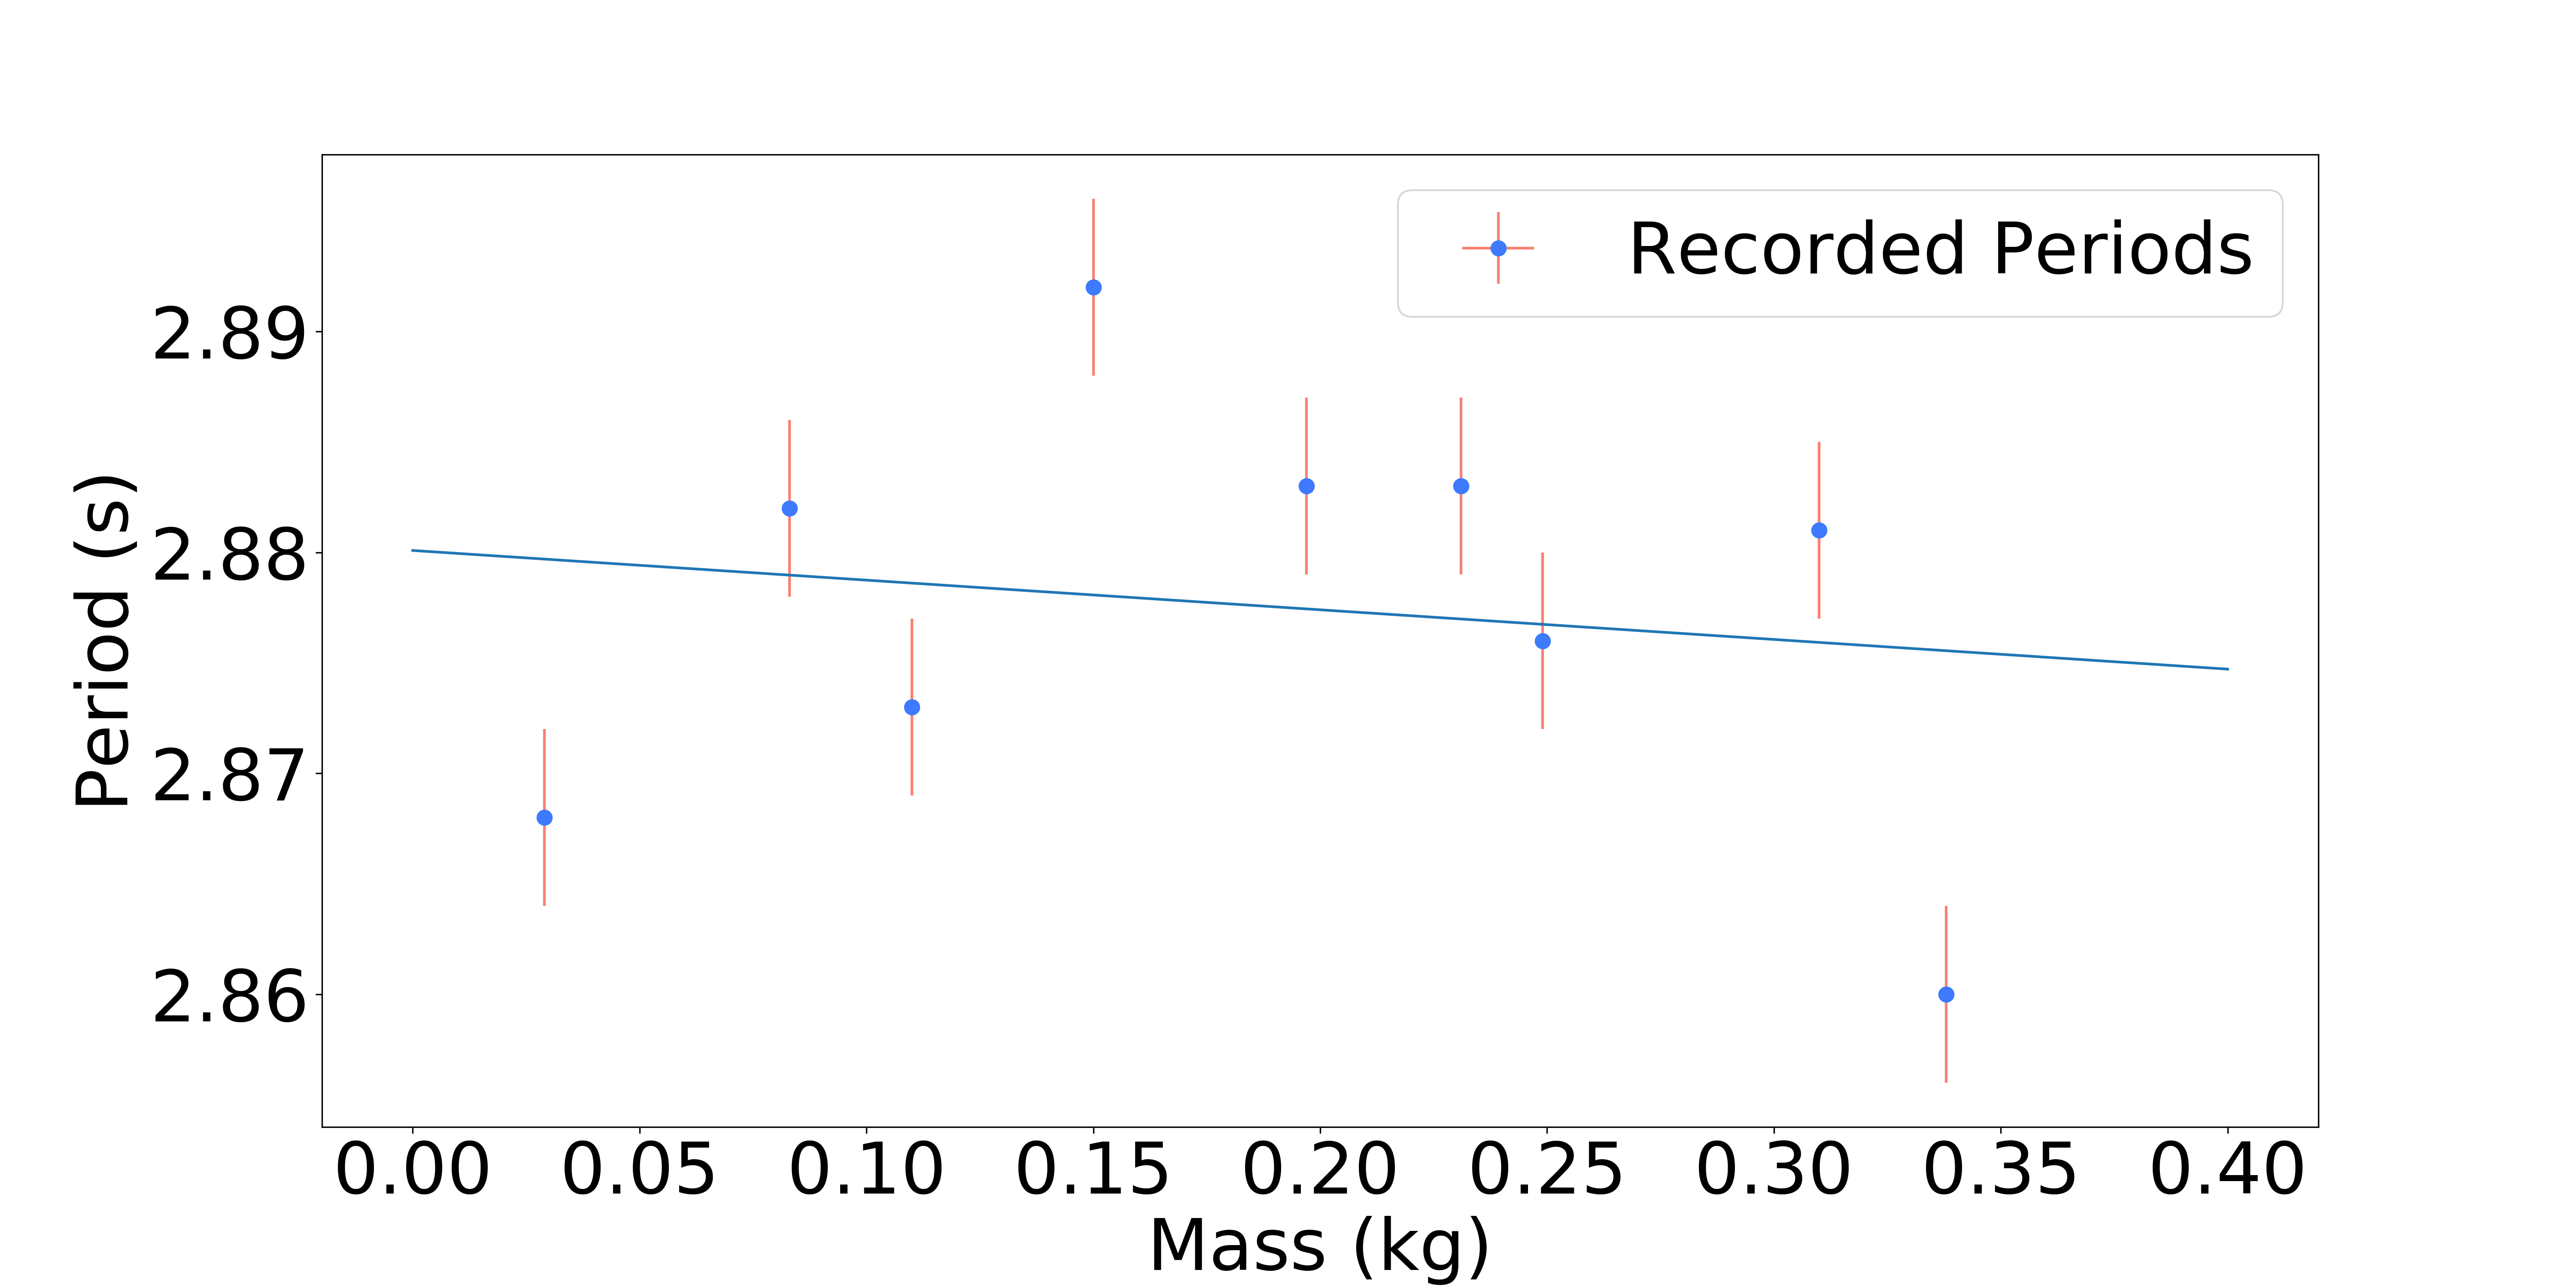
\includegraphics[width=\linewidth]{Figures/mass_simple.png}

    \caption{A plot of the period against the mass of the pendulum. Notice that the variations are similar in size to the uncertainties.}
    \label{fig:mass-simple}
\end{figure}
If a linear fit is used, the slope is given by:
\begin{equation}
    m = -0.01 \pm 0.03
    \label{eq:}
\end{equation}
which is effectively zero. It will be discussed later that the instrumentation is insensitive enough that any variation in the center of mass due to changing the water level will not be noticeable, so this behaviour is expected.% PLAN: GIVE SOLUTION TO DIFFERENTIAL EQUATION AND DO THE FIT
\section{Discussion}
\subsection{Amplitude Dependance}
\subsubsection{Uncertainty of Amplitude Intervals}
Demanding that the amplitude intervals have a range of $\Delta \theta = 0.2$ is quite accurate, even for large angles. If we assume the model is valid, then I am essentially finding the average period from $\theta_1$ to $\theta_1+\Delta \theta$, or:
\begin{equation}
    T_\text{avg} = \frac{1}{\Delta \theta}\int_{\theta_1}^{\theta_1+\Delta \theta} T_0\left(1+\frac{1}{16}\theta^2\right)\dd{\theta}
    \label{eq:}
\end{equation}
via experimental sampling. For the measured value of $T_0$ and using $\theta_1=-\frac{\pi}{2}$, I get that the average period should be around $T_\text{avg}=2.430 \pm 0.007\si{\second}$. I then let this average be equal to the linear approximation, which on the other hand would yield the period at the midpoint:
\begin{equation}
    T_\text{avg,approx} = T_0\left(1+\frac{1}{16}\left(\theta_1+\frac{\Delta \theta}{2}\right)^2\right)
    \label{eq:}
\end{equation}
giving $T_\text{avg,approx}=2.390 \pm 0.007 \si{\second}$. Here, the relative error reaches a maximum of $1.6\%$ at $\pi/2$. This is reasonable since the relative error using a quadratic approximation versus a quartic approximation gives a relative error of $1.9\%$, which has the same size.

\subsubsection{Impact of Q Factor}
Qualitatively, the $Q$ factor describes how slowly the system decays, so the higher the $Q$ factor, the more data points there are in each interval, which decreases the time uncertainty of each measurement.

A Q factor of $247\pm 2$ is sufficiently high such that for angles less than $70^\circ$, each interval has at least four data points, and for even smaller angles such as $35^\circ$, there were at least eight 10 data points.

Unfortunately, the decay at the very start was extremely rapid and only one measurement was able to be made for the initial angle. However, due to the high frame rate used, the uncertainty was still only $1\%$. It might be tempting to try to apply the $Q$ factor to the start of the motion, but it is only valid for small angles. At large angles, the effective $Q$ factor becomes smaller, and can drop by a factor of four.
\subsubsection{Uncertainties}
Overall, this experiment was conducted extremely well, with physical parameters such as the period agreeing with the predicted value. With the changes mentioned in the Introduction, several uncertainties were reduced:
\begin{itemize}
    \item Coupling Effects: There is no more rotation, so this effect has been eliminated completely.
    \item \textit{Tracker}: By nearly doubling the frame rate, and having a bottle that does not rotate, \textit{Tracker} had less error identifying where the pendulum was. I estimate this error to be one third the dimensions of the cap, which corresponds (as calculated in Python) to an average angular uncertainty of $0.3^\circ$ degrees.
\end{itemize}
The length uncertainty remains the same and is now the biggest source of uncertainty when determining the physical parameters such as the period. In the next experiment, I was able to carefully measure the center of mass of the bottle to a greater degree of accuracy by seeing how the period changes as the length of the rope fluctuates.
\subsubsection{Small Angle Approximation Validity}
In this section, we will check if the quadratic approximation
\begin{equation}
    T = 2\pi\sqrt{\frac{\ell}{g}}\left(1+\frac{1}{16}\theta_0^2\right)
    \label{eq:}
\end{equation}
is valid, and at which angles the simple harmonic oscillator (SHO) formula can be used:
\begin{equation}
    T = 2\pi\sqrt{\frac{\ell}{g}}
    \label{eq:}
\end{equation}
We can achieve this by attempting a quartic fit, as shown in figure \ref{fig:period-vs-amplitude-quartic}. A quartic fit gives the fit of:
\begin{equation}
    T = T_0\left(1+\alpha\theta_0+\beta\theta_0^2+\gamma \theta_0^3+\zeta \theta_0^4\right)
    \label{eq:}
\end{equation}
and parameters:
\begin{align}
    T_0 &= 2.14 \pm 0.01 \\ 
    \alpha &= 0.002 \pm 0.004 \\ 
    \beta &= 0.064 \pm 0.007 \\ 
    \gamma &= -0.006 \pm 0.003 \\ 
    \zeta &= 0.0029 \pm 0.0008
    \label{eq:}
\end{align}
As predicted, the coefficients of the odd powers $\alpha$ and $\gamma$ are close to zero, with their uncertainties being approximately the same as their nominal values. Meanwhile, the value of $\beta$ has improved to $0.064\pm 0.007$, which has a relative error of less than $3\%$! This is an improvement from the $7\%$ relative error when $\beta=0.0670 \pm 0.0007$ was used. Additionally, the value of $\zeta$ has a relative error of $19\%$ with respect to the theoretical value of $\zeta_\text{theory}=\frac{11}{3072}\approx 0.0036$.
\begin{figure}[!h]
    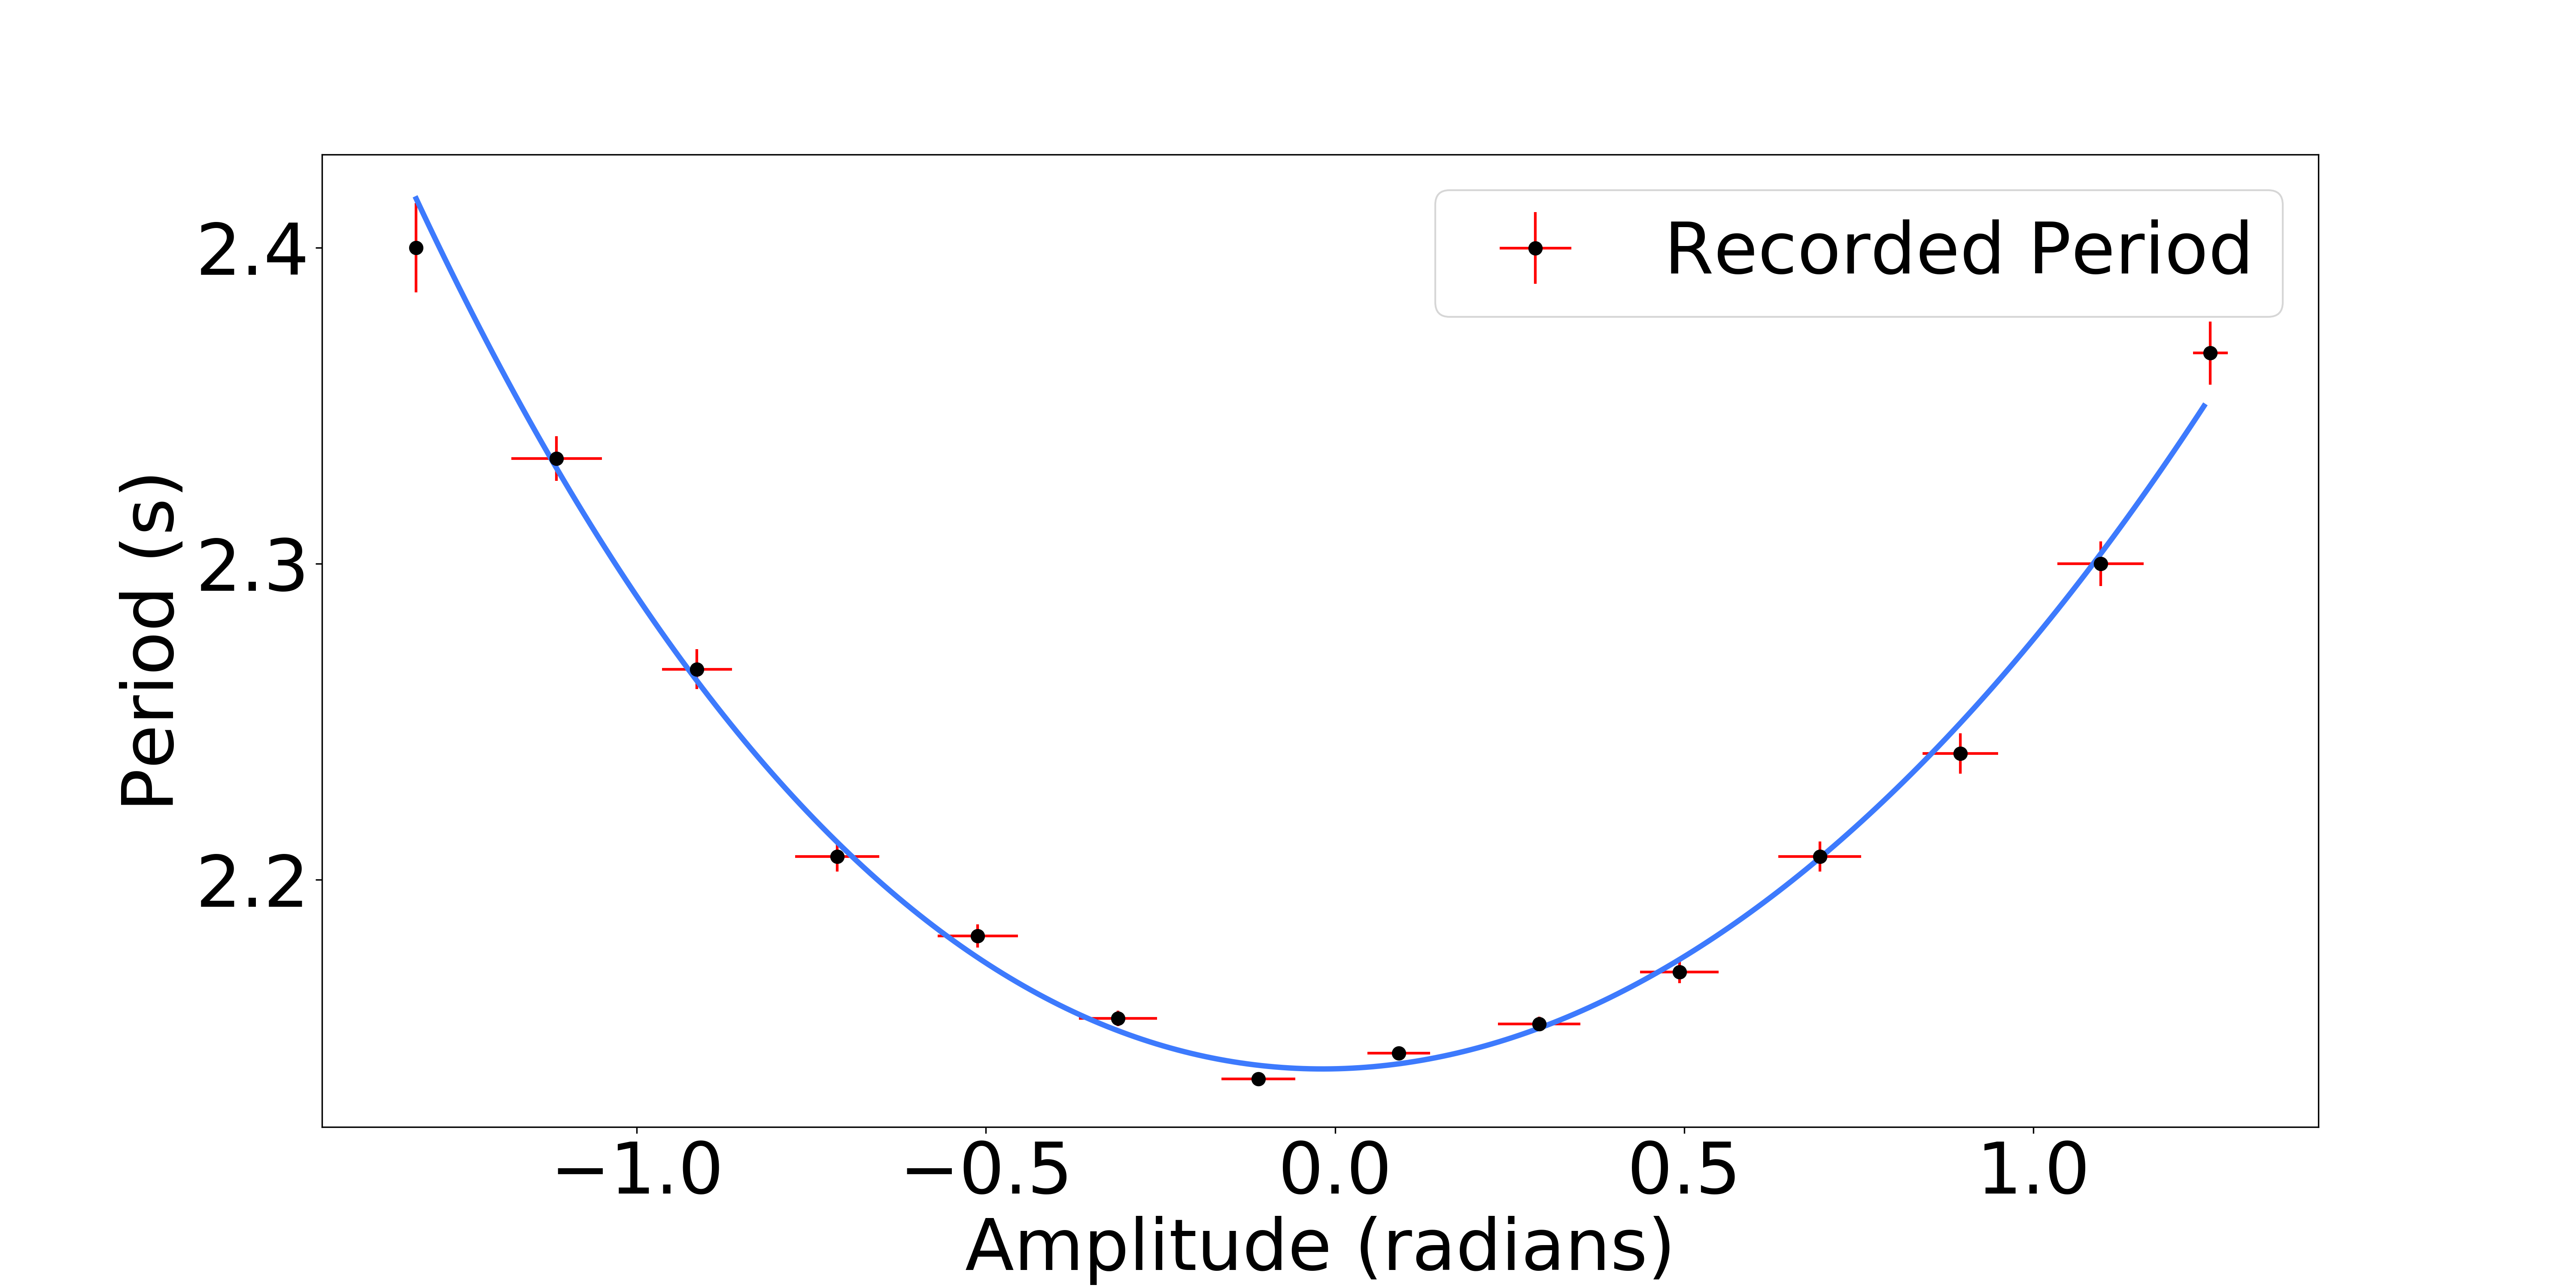
\includegraphics[width=\linewidth]{Figures/period-vs-amplitude-quartic.png}

    \caption{A plot of the period as a function of the amplitude, when fitted to a quartic function.}
    \label{fig:period-vs-amplitude-quartic}
\end{figure}
While this may seem like a large error, the theoretical value is actually within the statistical margins for $\zeta$. The likely values for $\zeta$ take on from $\zeta \in [0.0021,0.0037]$, and $\zeta_\text{theory}$ is contained in this range. I predict that if more accurate data was collected, especially at higher angles, then the nominal value of $\zeta$ will get closer to the predicted value and the uncertainties would decrease.

Since the coefficients become closer to their predicted value, this further supports that the model presented in equation \ref{eq:correct-model} is valid, which we can use to determine when we can use a quadratic model instead of a quartic model. We can do this by demanding the relative error in the period to be less than the time uncertainty divided by the period $\frac{\Delta t}{T} = 0.0023\si{\second}$, or:
\begin{equation}
    \frac{\frac{11}{3072}\theta^{4}}{1+\frac{1}{16}\theta^{2}+\frac{11}{3072}\theta^{4}} \le 0.0023
    \label{eq:}
\end{equation}
which gives the maximum angle to be $\theta_\text{max,quadratic}=0.911$ or $52.2^\circ$. Meanwhile, the maximum angle in which we can use the SHO formula instead of the quadratic approximation is given by when their relative error is under the time uncertainty as well:
\begin{equation}
    \frac{\frac{1}{16}\theta^{2}}{1+\frac{1}{16}\theta^{2}} \le 0.0023
    \label{eq:}
\end{equation}
which corresponds to an angle of $\theta_\text{max,SHO}=0.194$ or $11.1^\circ$. The relative error was chosen to be $\Delta T/T$ in an attempt to be as objective as possible. These angles represent the maximum angle at which the current apparatus can no longer detect a difference between the two models. Depending on the degree of precision needed, we may be happy with a relative error of $1\%$, in which case the angles at which a quadratic and SHO approximation can apply are $\theta_\text{max,quadratic}=76.2$ and $\theta_\text{max,SHO}=28.0^\circ$, respectively.
\subsection{Q Factor}
\subsubsection{Uncertainties}
All uncertainty analysis was done using the Python \textit{uncertainties} package\cite{uncertainties}. The time uncertainty for each measurement is determined by the frame rate, which although was filmed in 60fps, but was processed in 30fps for practical purposes. The primary purpose of the high frame rate was to increase the clarity of each frame. Nevertheless, the time uncertainty of half a frame $\Delta t \approx 0.02\si{\second}$ ends up being negligible when we divide by the total number of swings, which is approximately $262\pm 2$ to get $\frac{\Delta t}{262}\approx 6 \times 10^{-5}$.

The \textit{Tracker} software was able to track the location of the cap at all times. Sometimes it would track the left side of the cap while other times it would track the right side. I estimate the relative uncertainty for each measurement to be around $\Delta x \approx 1.4\si{\centi\meter}$, which is the radius of the cap. Python was then able to propagate this error to calculate the uncertainty in the angle, which has a typical value of $\Delta \theta \approx 0.007 \approx 0.4\si{\degree}$. While this is not a big problem early on, the relative error slowly becomes larger and the maximum relative error becomes $0.12$, which is around three orders of magnitude larger than the time uncertainty in the frames. Since the period is independent of the amplitude, this will not affect the period, but will affect the time constant.

The effective distance to the center of mass also has some uncertainty. We can perform a naive estimation of the center of mass as:
\begin{equation}
    (11.1+2.5) - \frac{1}{2}\left(\frac{(11.1\si{\centi\meter} + 2.5 \si{\centi\meter})+(2.5\si{\centi\meter})}{2}\right) \approx 7 \pm 1\si{\centi\meter}
    \label{eq:}
\end{equation}
from the cap, which is the point of attachment of the string. This comes from a simple max/min calculation assuming the trapezoidal pyramid was absent (for the max calculation), and assuming the trapezoidal pyramid was a rectangular prism (for the min calculation). This leads to an uncertainty in the period of $\Delta T = 0.008\si{\second}$ which is around two orders of magnitude larger than the uncertainty caused by the time. Since $Q$ is proportional to the period, the relative uncertainty in the $Q$ factor will be very similar.

We have also made the claim that the $Q$ value obtained from counting oscillations gives the upper bound while the $Q$ value obtained from the line of best fit gives the lower bound. From figure \ref{fig:amplitude-vs-time}, it can be seen that the best fit underestimates the initial angles as well as the final angles, which suggests that the actual decay happens much slower than predicted. Since the $Q$ factor is a measure of how slowly a dampened harmonic system decays, it makes sense that the value obtained from the fit is smaller than the fit obtained from counting the data. However, an exponential fit that passes through the points of interest will skew the other parts of the graph to be not accurate. As a result, if we are assuming a linear drag force, then the $Q$ factor will be somewhere between these two extremes. However, as the next section will explore, a decaying exponential enveloping function is not valid, and thus there is no use assigning a single value as the $Q$ factor.

\subsubsection{Linear or Quadratic Drag}
It appears that while the exponential model is a good approximation, the enveloping function was not entirely linear when the natural logarithm of the amplitudes were plotted. This gives sufficient reason to look into if the drag may not be linear with respect to velocity, but instead quadratic, given by the drag equation:
\begin{equation}
    F_d = -\frac{1}{2}c_d\rho A|v|v = -\beta |v|v
    \label{eq:}
\end{equation}
where $\rho$ is the density of air, $A$ is the cross sectional area and $c_d$ is the drag coefficient, which we have all clumped together in $\beta$. Unfortunately, the differential equation for quadratic drag does not have a nice closed form. However, by assuming that the change in amplitude is small over a small time interval, we can approximate the enveloping function as\cite{Hauko}:
\begin{equation}
    \theta = \displaystyle \frac{\theta_0}{1+\alpha T}
    \label{eq:}
\end{equation}
where:
\begin{equation}
    \alpha \equiv \frac{4\beta \omega \theta_0}{3\pi}
    \label{eq:}
\end{equation}
However, this appears to also not be the entirely correct model. The value of $\alpha$ can be determined by plotting $\frac{1}{\theta}$ as a function of $t$:
\begin{equation}
    \frac{1}{\theta} = \frac{1}{\theta_0}+\frac{\alpha}{\theta_0}t
    \label{eq:}
\end{equation}
and the value of $\theta_0$ and $\alpha$ can be read off of the y intercept and slope to get $\alpha = 0.0102 \pm 0.00023$ and $\theta_0=0.368 \pm 0.008$. Qualitatively, as seen in figure \ref{fig:quad-amplitude-vs-time}, the data conforms to a quadratic model of air resistance much better than a linear model. 
\begin{figure}[h]
    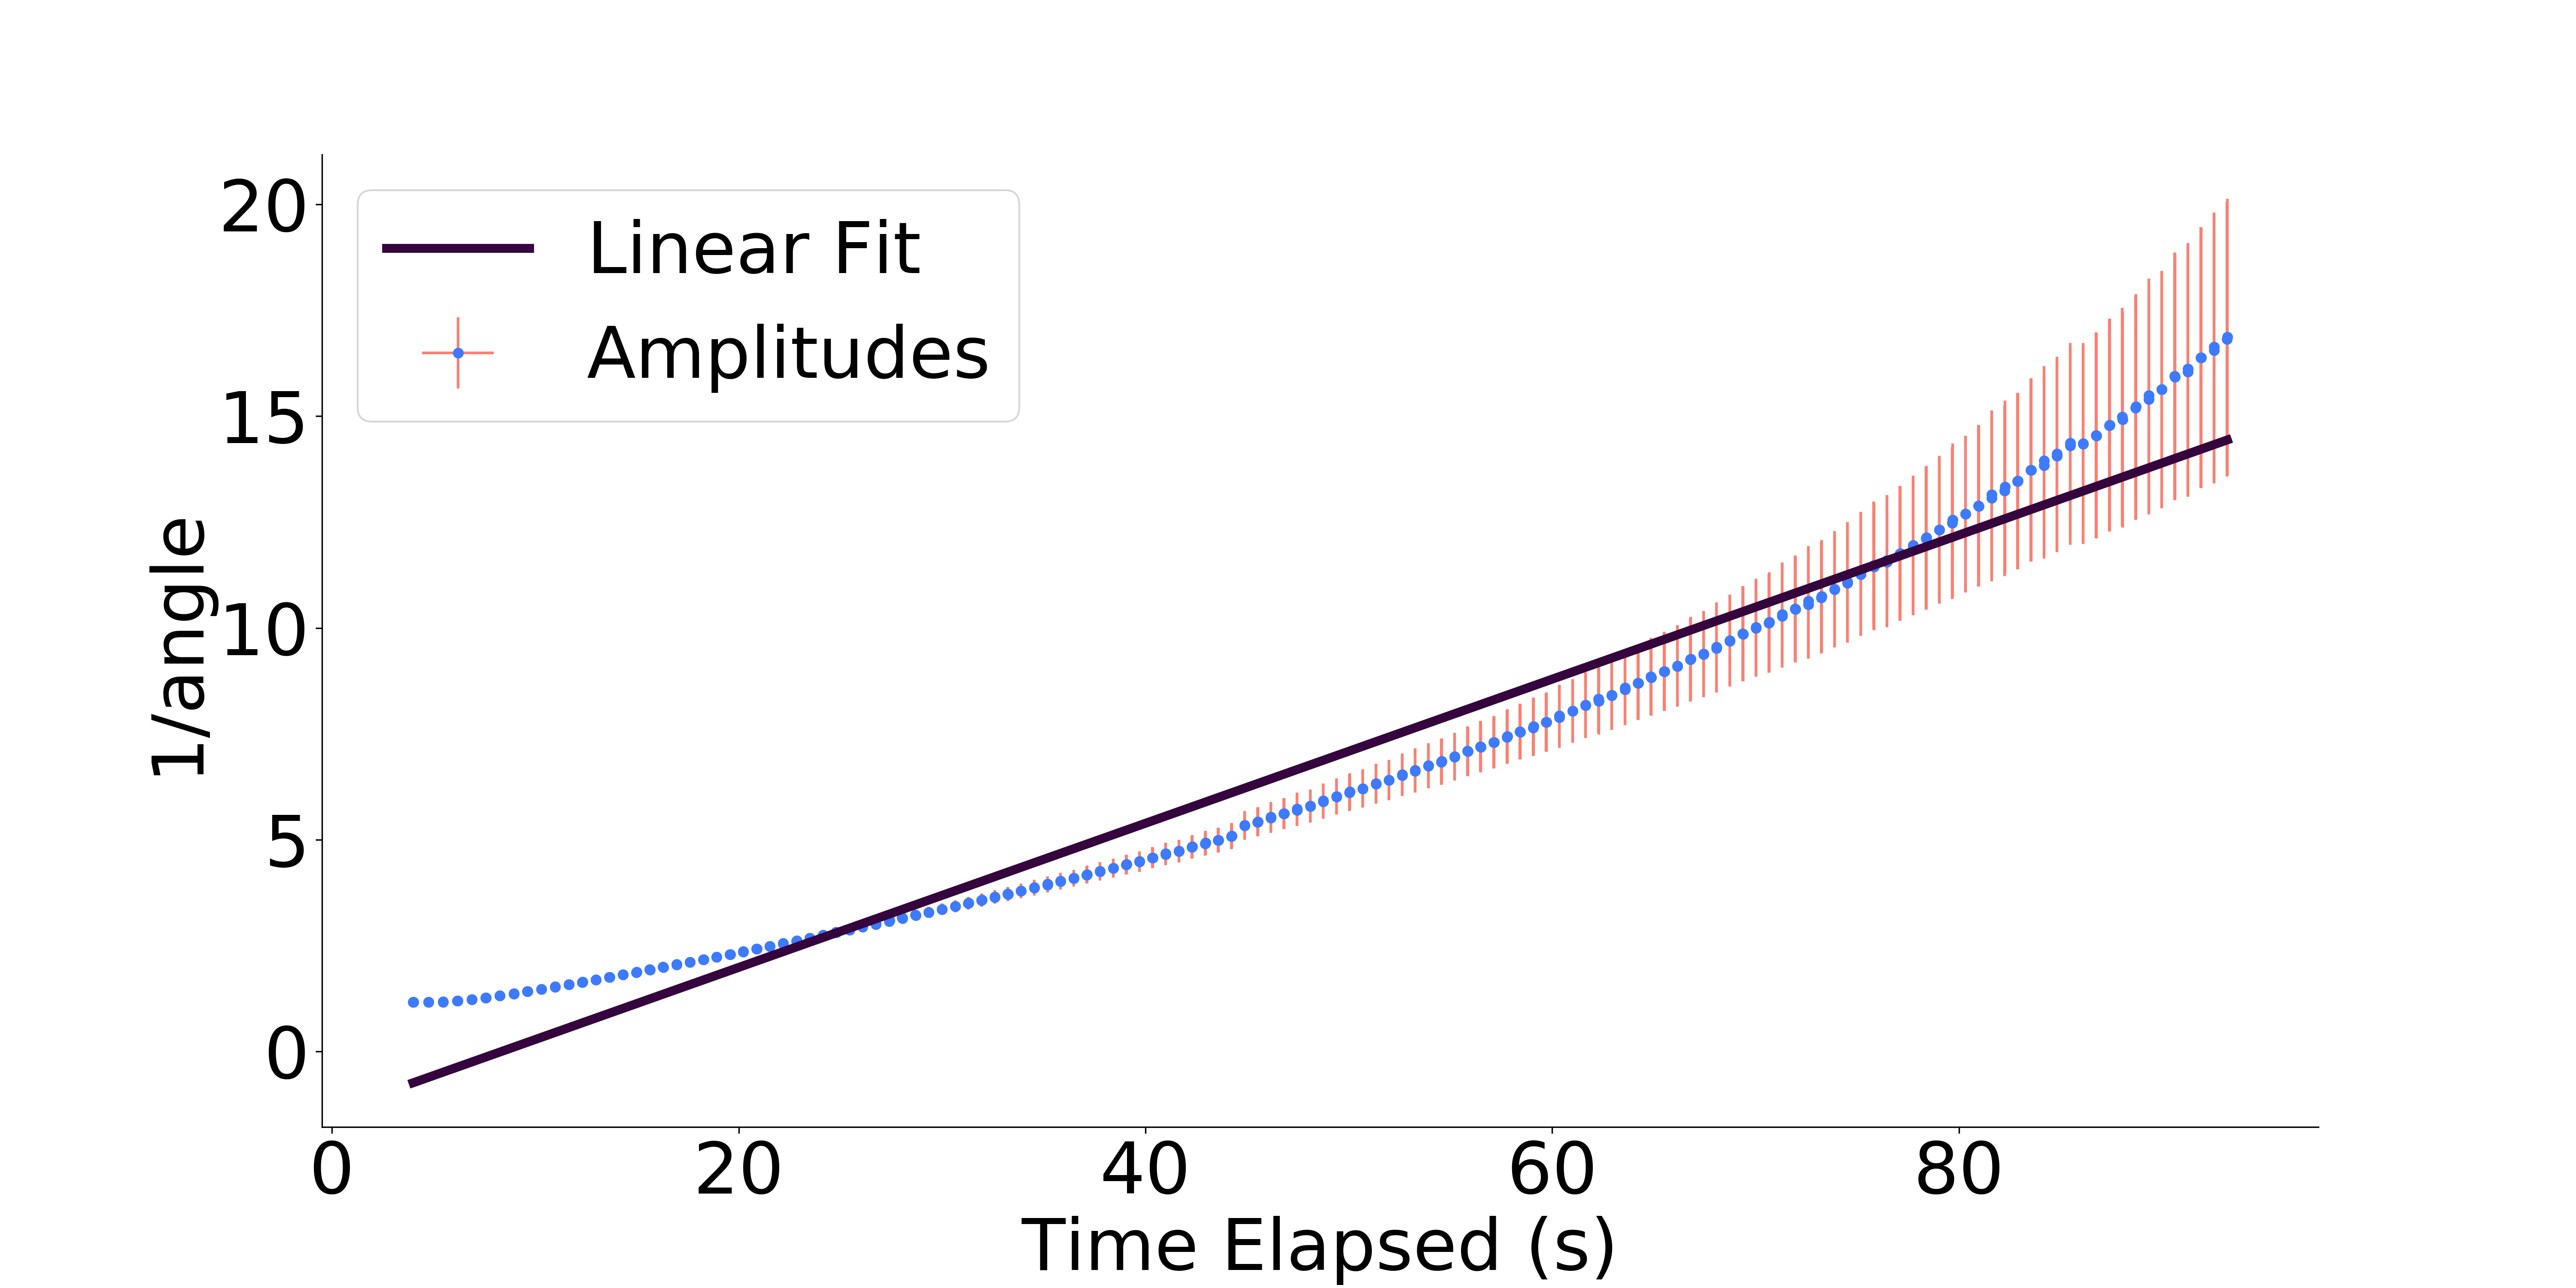
\includegraphics[width=\linewidth]{figures/quadratic-amplitude-vs-time-fitted.png}

    \caption{A plot of the $1/\theta$ with the line of best fit. A clear nonlinear pattern is shown, suggesting that the drag is not entirely quadratic in nature.}
    \label{fig:quad-amplitude-vs-time}
\end{figure}
However, it is possible for the drag to be a combination of the two. Quadratic drag typically occurs for streamline flow (e.g. laminar flow) while linear drag can be an approximation for turbulent flow. Turbulence is a tricky concept, and way beyond the scope of this lab.

With that being said, there is some justification behind this. In the linear approximation in the semi-log plot show in figure \ref{fig:amplitude-vs-time}, the line of best fit under-approximates the angle initially. If the drag started off as quadratic, the amplitude versus time graph will scale like $\theta \propto \frac{1}{1+t}$, which will lead to higher angles than if the amplitudes scaled like $\theta \propto e^{-t}$, assuming that both are normalized to obtain the same values for small values of $t$.

It is interesting to note however, that in other experiments with a longer string length, the flow seemed to exhibit laminar patterns for the majority of the motion and the reciprocal fit was extremely good. More experimentation with carefully controlled conditions need to be performed to see which form of flow is truly more dominant and whether this depends on the string length. 
\subsection{Length Dependance}
The precision of all measurements were extremely high. Since there were over $200$ data points, but they were merged together in groups of five, the time uncertainty for the period will be negligible. The length measurements were done by a computer, and ideally, they should be overestimated the same amount of times they are underestimated such that the average length is very precise as well. This is why error bars were barely noticeable. However, even though the experimental results seem to agree with the theoretical predictions, they were still off by a little bit. For example, the predicted slope in figure \ref{fig:plot-2} had a minimum of $4.01\si{\second\squared\per\meter}$ while the value for the experimental slope had a maximum value of $4.00\si{\second\squared\per\meter}$. These small dispecrancies are still worthy of investigation, and can be caused by two main things:
\begin{itemize}
    \item Systematic error: While measurements were very precise, they could all be consistently off the true value by some fixed amount.
    \item Incorrect model: The model introduced in the hypothesis may not be entirely correct and there can be external factors that have a larger impact than previously thought.
\end{itemize}
\subsubsection{Systematic Errors}
The largest form of systematic error would be the measurement of the length of the pendulum. However, if the length of the string was consistently measured to be smaller than the true value by a certain amount $x$, then the distance from the endpoint of the string to the center of mass of the bottle would be larger by the same amount $x$ such that $\ell_\text{cm}$ is a constant. Furthermore, shifting the length by a fixed amount does not affect the value of the slope, only the $y$ intercept.

Another way the string could be measured incorrectly is an incorrect scaling factor to convert from pixels to meters. While a ruler was placed in the background to set a scale, that scale was found to be inaccurate and only served to ensure the final numbers were in the right order of magnitude. An additional scaling factor was manually determined by measuring the initial $1.985\si{\meter}$ string to $\pm 0.003\si{\centi\meter}$ accuracy. This fairly large uncertainty comes from the fact that multiple measurements had to be made and the string was attached at an angle such that the vertical distance the string extends is not equal to the length of the string. This means that the length of the string could be scaled up or scaled down by a factor of 
\begin{equation}
    \frac{\ell_\text{measured}}{\ell_\text{true}} = \left(1 \pm \frac{0.003}{1.98}\right)
    \label{eq:}
\end{equation}
This means that if the slope is $m$, then it adds on another uncertainty of around:
\begin{equation}
    \delta m = m\left(\frac{0.003}{1.98}\right) \approx 0.01 \si{\second\squared\per\meter}
    \label{eq:}
\end{equation}
which is approximately the difference between the upper and lower bounds of the theoretical value and the experimental value for the slope of the linearized graph.
\subsubsection{Other Factors}
Contradictions appear to arise when the original function is fit to the function:
\begin{equation}
    T = \sqrt{\alpha \cdot \frac{I+\ell_\text{cm}^2}{\ell_\text{cm}}}
    \label{eq:moment of inertia}
\end{equation}
to determine the value of $I$, which is the specific moment of inertia. This is done in \ref{fig:normal-complex}.
\begin{figure}[!h]
    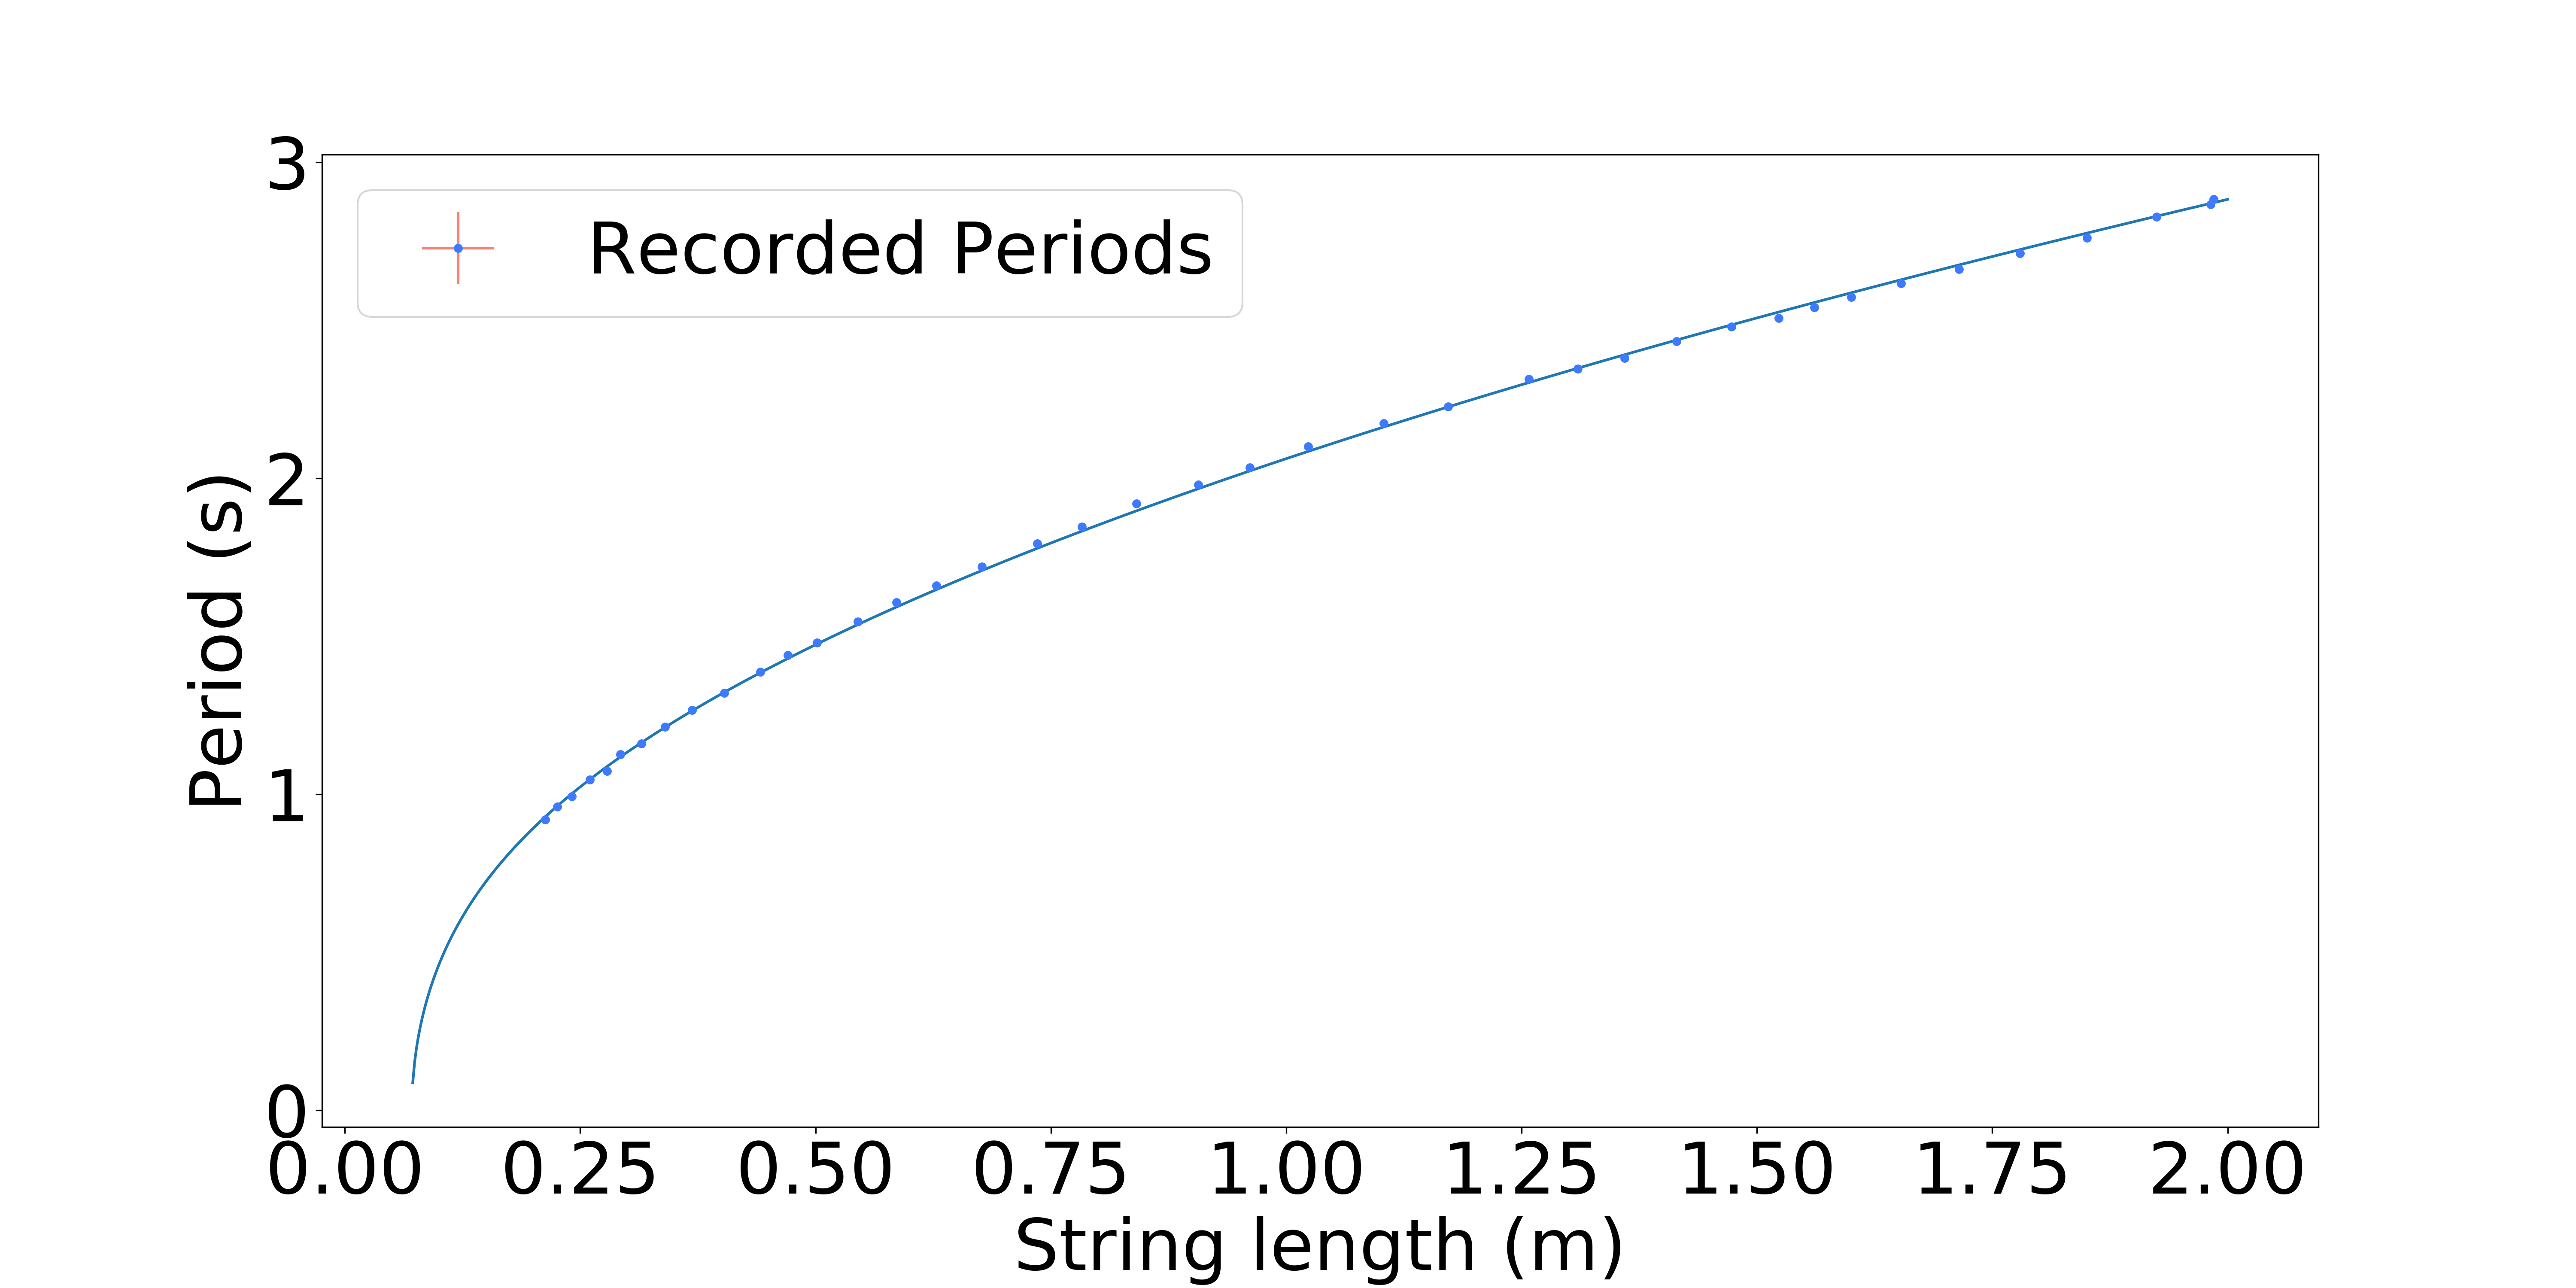
\includegraphics[width=\linewidth]{Figures/normal_complex.png}

    \caption{A plot of the period against the length of the center of mass of the pendulum. Notice that the plot visually looks much more accurate than that of \ref{fig:linear-1}.}
    \label{fig:normal-complex}
\end{figure}
The value for $\alpha$ and $I$ are given as:
\begin{align}
    \alpha &= 4.015 \pm 0.008 \si{\second\squared\per\meter}\\ 
    I &= -0.0228 \pm 0.0007 \si{\meter\squared}
\end{align}
Note that the theoretical value of $\alpha$ is given in equation \ref{eq:mtheory} as $\alpha_\text{theory}=4.03 \pm 0.02 \si{\second\squared\per\meter}$. Here, the experimental value is closer to the theoretical model than that shown in figure \ref{fig:plot-2}. However, the moment of inertia takes on a negative value, which is simply impossible! The uncertainty is also very low, so this suggests that there is something wrong with the physical model. I claim that this is due to neglecting the effects of air resistance. As shown earlier, the true angular frequency of an underdampened pendulum is:
\begin{equation}
    \omega = \sqrt{\omega_0^2\left(1-\left(\frac{2}{Q}\right)^2\right)}
    \label{eq:omegalol}
\end{equation}
However, both air resistance and an extra moment of inertia will tend to increase the period, not decrease it. Therefore, there is some mechanism that is adding in energy. One possible mechanism that can accomplish this is that the manual rising of the string could be increasing the angular speed. I will investigate how large of an effect this is by writing out the rotational equation of motion as:
\begin{equation}
    \frac{dL}{dt} = \frac{d}{dt}\left(m \ell^2 \omega\right) = -mg\ell\sin\theta
    \label{eq:}
\end{equation}
Applying the product rule, this gives:
\begin{align}
    2m\ell\omega \frac{d\ell}{dt} + \frac{d\omega}{dt}m\ell^2 &= -mg\ell\sin\theta \\ 
    \frac{d^2\theta}{dt^2} &= -\frac{g}{\ell}\theta + \frac{2\dot{\ell}}{\ell}\dot{\theta}
    \label{eq:}
\end{align}
The average value for $\dot{\ell}$ is $\dot{\ell}_\text{avg}=0.00440 \pm 0.00001 \si{\meter\per\second}$. The effective damping coefficient is now negative, which means that the period should be shorter than expected. Similar to \ref{eq:omegalol}, we can derive the period as:
\begin{equation}
    T = T_0\sqrt{\left(1-\frac{1}{\omega_0^2}\left(\frac{\dot{\ell}}{\ell}\right)^2\right)}
    \label{eq:}
\end{equation}
Comparing this to equation \ref{eq:moment of inertia}, which can be written as:
\begin{equation}
    T = T_0\sqrt{\left(1+\frac{I}{\ell^2}\right)}
    \label{eq:}
\end{equation}
We can derive the specific moment of inertia to then be:
\begin{equation}
    I = -\frac{\ell \dot{\ell}^2}{g} \approx -5 \times 10^{-6} \si{\meter\squared}
    \label{eq:}
\end{equation}
which is essentially negligible. It appears that there is no straightforward explanation to why the theoretical model overestimates the period. Accounting for a nonzero moment of inertia and air resistance damping effects only leads to an increase in the period, not a decrease. More experimentation needs to be done to pin down the reason behind this dispecrancy. As a result, it is likely this is due to a systematic error of how certain measurements were made, that were not included in the previous section. For example, perhaps I have overestimated the precision at which the string length can be measured. It is recommended that the experiment be completed again, including any or a combination of the following modifications:
\begin{itemize}
    \item Using a small but heavy mass.
    \item Taking period measurements in multiple independent methods.
    \item Changing the string length in a different way.
    \item Measuring the string length in multiple independent methods.
\end{itemize}
\subsection{Mass Dependance}
\subsubsection{Systematic Errors}
Many systematic errors that appear in the length dependance are not significant when looking at the length dependance. As long as the length of the string can be measured precisely, it does not matter how accurately it is measured. For example, it is perfectly acceptable even if every measurement of the length is larger than the true amount by $5\si{\centi\meter}$, as long as this error is consistent. This is because I am looking if there is a trend when the mass is changed.

A kitchen scale was used to measure the mass of the bottle, which has a precision of $\pm 0.5\si{\gram}$. Timing was done with a stopwatch and from the mini experiment described in the Introduction, I found myself to stop the stopwatch earlier roughly the same amount of times I stopped it late. As a result, it is very unlikely that there are any systematic errors that could affect the measurements.

\subsubsection{Other Factors}
Since the mass is changed by removing or adding water from the bottle, the center of mass is able to change. I can approximate the bottle as a rectangular prism with a height of $13.2 \pm 0.1 \si{\centi\meter}$ and a base consisted of a square with side lengths $5.0 \pm 0.1 \si{\centi\meter}$ such that the total volume is around $330\si{\milli\meter}$. An empty bottle weighs $29 \pm 0.5 \si{\gram}$ and assuming the mass distribution is constant, the center of mass of the bottle when the water is at a height $h$ is given by:
\begin{equation}
    d_\text{cm} = \frac{\left(\rho(5.0)^2h\right)\frac{h}{2} + 29\left(\frac{13.2}{2}\right)}{29+\left(\rho(5.0)^2h\right)}
    \label{eq:}
\end{equation}
which reaches a maximum of $d_\text{cm,max}=6.6\si{\centi\meter}$ and a minimum of $d_\text{cm,min}=2.9\si{\centi\meter}$ such that the effective uncertainty of the center of mass can be seen as $\delta \ell_\text{cm}=6.6-2.9 = 0.037\si{\meter}$. The relative uncertainty in the period is given by:
\begin{equation}
    \frac{\delta T}{T} \approx \frac{\delta \ell_\text{cm}}{2\ell_\text{cm}} \implies \delta T = \frac{\delta \ell}{2\sqrt{g\ell_\text{cm}}}
    \label{eq:}
\end{equation}
If approximately a two meter long string is used, then the uncertainty in the period is:
\begin{equation}
    \delta T \approx 0.004\si{\second}
    \label{eq:}
\end{equation}
My reaction speed to a predictable visual event is $0.04 \pm 0.02\si{\second}$, which was obtained by attempting to stop the stopwatch on the iPhone ``clock app'' every time the second hand crosses the five second mark. If ten oscillations are used to determine the period, then the uncertainty in the period measurement will be on the same order of magnitude as $\delta T$. Therefore, even though the center of mass of the pendulum will be changing, it is very likely no trend will be seen.

Another contributing factor could be air resistance. From equation \ref{eq:omegalol}, we can show that the period of the pendulum is:
\begin{equation}
    T = T_0\sqrt{1+\left(\frac{2}{Q}\right)^2}
    \label{eq:}
\end{equation}
Since $Q \equiv \frac{m}{b}\sqrt{\frac{\ell}{g}}$, decreasing the mass effectively decreases the $Q$ factor by the same proportion. The pendulum used has an average center of mass of $\ell_\text{cm}=2.015 \pm 0.003 \si{\meter}$, so the $Q$ factor is around:
\begin{equation}
    Q_\text{new} = Q_\text{before}\sqrt{\frac{201.5}{115}} = 433 \pm 4
    \label{eq:}
\end{equation}
where the quality factor at a length of $\ell_\text{cm}=115\si{\centi\meter}$ was $Q_\text{before}=247 \pm 2$. This means that for a mass $m$, the quality factor is:
\begin{equation}
    Q = \frac{m}{338} \cdot \left(443 \pm 4\right)
    \label{eq:}
\end{equation}
For the lowest mass, this gives a $Q$ factor of approximately:
\begin{equation}
    Q = 37.1 \pm 0.3
    \label{eq:}
\end{equation}
This means that the relative error in the period uncertainty is around:
\begin{equation}
    \delta T = T\left(\frac{2}{Q^2}\right) = 0.004
    \label{eq:}
\end{equation}
which also coincidentally happened to be within my measurement error. Therefore, the mass does not greatly impact the motion of the pendulum. The fluctuations could very easily be caused by external factors such as a changing center of mass and air resistance. The next steps would be to develop a method to lower measurement uncertainties such that these other factors can be quantified, measured, and accounted for. One possible method is to poke a small hole such that water slowly drains out. However, I will need to be careful as large holes will cause the water to drain out too quickly and small holes will cause surface tension to have a large effect.
\section{Conclusion}
In conclusion, it appears that simple dampened harmonic motion is not the best model that describes a swinging pendulum. The air resistance isn't necessarily $F_d = -bv$, the restoring torque isn't necessarily proportional to the angular displacement. The instructions have also approximated the pendulum as a point mass, which was shown to also not be true.

The irregular shape of the pendulum in the form of a water bottle could have lead to other unexpected effects. For future experiments, it would be ideal to have a more aerodynamic shape to prevent turbulence, and allows for a careful analysis of how mass affects the period without changing the location of the center of mass.
\onecolumngrid
\bibliography{citations}

\newpage
\appendix
\section{Solution to Linear Drag}
\noindent To solve the differential equation:
\begin{equation}
    \ddot{\theta}+2\pi Q\dot{\theta}+4\pi^2\theta=0
    \label{eq:}
\end{equation}
where derivatives are taken with respect to the dimensionless factor $T$, we can guess a general solution in the form of $Ae^{\alpha T}$ to get:
\begin{equation}
    \alpha^2Ae^{\alpha T}+2\pi Q\alpha Ae^{\alpha T}+4\pi^2Ae^{\alpha T}=0 \implies \alpha^2+2\pi Q\alpha+4\pi^2 = 0
    \label{eq:}
\end{equation}
This gives a quadratic in $\alpha$ where the solution is:
\begin{equation}
    \alpha = \frac{-2\pi Q \pm \sqrt{4\pi^2Q^2-16\pi^2}}{2}= -\pi Q\pm \pi\sqrt{Q^2-4}=-\pi Q\left(1\pm\sqrt{1-\left(\frac{2}{Q}\right)^2}\right)
    \label{eq:}
\end{equation}
Since we have a linear equation, the solution will consist of a linear combination:
\begin{equation}
    \theta(t)=Ae^{\alpha_1t}+Be^{\alpha_2t}=e^{-\pi Q T}\left(Ae^{\sqrt{1-(2/Q)^2}}+Be^{\sqrt{1-(2/Q)^2}}\right)
    \label{eq:}
\end{equation}
If we define $i\Omega=\sqrt{1-\left(\frac{2}{Q}\right)^2}$, then we can write the general solution as:
\begin{equation}
    \theta(t)=Ce^{-\pi QT}\cos\left(\Omega T+\phi\right)
    \label{eq:}
\end{equation}
as desired, where the identity:
\begin{equation}
    Ae^{-i\Omega T}+Be^{i\Omega T}=C\cos\left(\Omega T+\phi\right)
    \label{eq:}
\end{equation}
was used.
\section{Python Script and Data}
The script was written in Python through a Jupyter notebook, which is available to be viewed \href{https://github.com/QiLinXue/pendulum-labs}{here}. It consists brief descriptions of the code, as well as descriptions of how optical corrections were done. Automatic error propagation is included.

For practical reasons, I cannot include over the $200,000$ data points in this report, but they are made available in the link above. It consists of three columns: time, $x$-position, and $y$-position. The origin is set to the equilibrium position of the pendulum.
\end{document}